%
% File emnlp2016.tex
%

\documentclass[11pt,letterpaper]{article}
\usepackage[letterpaper]{geometry}
%camera-ready version
\usepackage[hyperref]{emnlp2018}
\aclfinalcopy
\usepackage{times}
\usepackage{latexsym}
\usepackage{amsmath}
\usepackage{appendix}
% use for left-aligned equation
%\usepackage[fleqn]{amsmath}
\usepackage{multirow}
\usepackage{url}
\makeatletter
% URL fixing
%\newcommand{\@BIBLABEL}{\@emptybiblabel}
\newcommand{\@emptybiblabel}[1]{}
\makeatother
%\usepackage[hidelinks,draft]{hyperref}
% URL fixing
\DeclareMathOperator*{\argmax}{argmax}
\DeclareMathOperator*{\argmin}{argmin}
\setlength\titlebox{6.5cm}    % Expanding the titlebox
\usepackage{color}
\usepackage{comment}
\usepackage{graphicx}
\usepackage[T1]{fontenc}
\usepackage{subcaption}
\usepackage{enumitem}
\usepackage{algorithm}
\usepackage{booktabs}
%\usepackage{cleveref}
\usepackage[noend]{algpseudocode}
%\parskip 0pt

\usepackage[all]{nowidow}
%\raggedbottom

% fancy symbol for section reference
\renewcommand{\subsectionautorefname}{\S}
\renewcommand{\sectionautorefname}{\S}
%% replace "section" with symbol
%\crefname{section}{�}{��}

% To expand the titlebox for more authors, uncomment
% below and set accordingly.
% \addtolength\titlebox{.5in}    

\newcommand\BibTeX{B{\sc ib}\TeX}
\newcommand{\example}[1]{\textit{#1}}
\newcommand{\gloss}[1]{``#1''}
\newcommand{\ian}[1]{{\color{magenta}(#1 - I)}}
\newcommand{\jacob}[1]{{\color{blue}(#1 - J)}}
% line break in cell
\newcommand{\specialcell}[2][c]{%
  \begin{tabular}[#1]{@{}l@{}}#2\end{tabular}}
\newcommand{\etal}{\emph{etal.}}
\newcommand{\var}[1]{\mathrm{#1}}
\newcommand{\set}[1]{\mathcal{#1}}
\newcommand{\model}[1]{\texttt{#1}}

%% reduce space after figure captions
%\setlength{\belowcaptionskip}{2pt}

%% squishing paragraphs
%\renewcommand{\paragraph}{%
%  \@startsection{paragraph}{4}%
%  {\z@}{2ex \@plus 1ex \@minus .2ex}{-1em}%
%  {\normalfont\normalsize\bfseries}%
%}

% prevents footnotes from breaking across columns
\interfootnotelinepenalty=10000

\title{Making ``fetch'' happen: The influence of social and linguistic context on nonstandard word growth and decline}

% Author information can be set in various styles:
% For several authors from the same institution:
% \author{Author 1 \and ... \and Author n \\
%         Address line \\ ... \\ Address line}
% if the names do not fit well on one line use
%         Author 1 \\ {\bf Author 2} \\ ... \\ {\bf Author n} \\
% For authors from different institutions:
% \author{Author 1 \\ Address line \\  ... \\ Address line
%         \And  ... \And
%         Author n \\ Address line \\ ... \\ Address line}
% To start a seperate ``row'' of authors use \AND, as in
% \author{Author 1 \\ Address line \\  ... \\ Address line
%         \AND
%         Author 2 \\ Address line \\ ... \\ Address line \And
%         Author 3 \\ Address line \\ ... \\ Address line}
% If the title and author information does not fit in the area allocated,
% place \setlength\titlebox{<new height>} right after
% at the top, where <new height> can be something larger than 2.25in

% add authors
\author{Ian Stewart and Jacob Eisenstein \\
School of Interactive Computing \\
Georgia Institute of Technology \\
Atlanta, GA 30318 \\
\url{{istewart6,jacobe}@gatech.edu}
}

\date{}

\begin{document}

\maketitle

\begin{abstract}
In an online community, new words come and go: today's \example{haha} may be replaced by tomorrow's \example{lol}. 
Changes in online writing are usually studied as a social process, with innovations diffusing through a network of individuals in a speech community.
But unlike other types of innovation, language change is shaped and constrained by the grammatical system in which it takes part.
To investigate the role of social and structural factors in language change, we undertake a large-scale analysis of the frequencies of nonstandard words in Reddit.
Dissemination across many linguistic contexts is a predictor of success: words that appear in more linguistic contexts grow faster and survive longer.
Furthermore, social dissemination plays a less important role in explaining word growth and decline than previously hypothesized.

\end{abstract}

\section{Introduction}

\textit{Stop trying to make ``fetch'' happen! It's not going to happen!} -- Regina George (\emph{Mean Girls}, 2005) \vspace{8pt}

With the fast-paced and ephemeral nature of online discourse, language change in online writing is both prevalent~\cite{androutsopoulos2011} and noticeable~\cite{squires2010enregistering}. 
In social media, new words emerge constantly to replace even basic expressions such as laughter: today's \example{haha} is tomorrow's \example{lol}~\cite{tagliamonte2008}. 
%The rise of such lexical innovations may reflect social trends in an online community such as the turnover of new members or the response to a content ban~\cite{danescu2013,chancellor2016moderation}. 
%The reasons for such changes are various: adopting new words may be used to signal familiarity with the latest trends in a community~\cite{bucholtz1999}, 
%%they may represent the orthographic representation of an existing spoken vernacular~\cite{eisenstein2015systematic} 
%or they may even result from an exogenous shock, such as the censorship of related terms~\cite{chancellor2016moderation}.
%But while analysis of specific causes for change can offer insights, we must also address a more basic set of questions. 
Why do some nonstandard words, like \example{lol}, succeed and spread to new contexts, while others, like \example{fetch}, fail to catch on? 
Can a word's growth be predicted from patterns of usage during its early days?

Language change
%, and lexical change in particular, 
can be treated like other social innovations, such as the spread of hyperlinks~\cite{bakshy2011everyone} or hashtags~\cite{romero2011differences,tsur2015}.
A key aspect of the adoption of a new practice is its \emph{dissemination}: is it used by many people, and in many social contexts?
%\newcite{altmann2011} compute dissemination across online newsgroups, finding that words with high early diffusion tend to succeed.
High dissemination enables words to achieve greater exposure among social groups~\cite{altmann2011}, and may signal that the innovation is positively evaluated.

%But while language change shares some properties with other social innovations, it is also bound by the constraints of the language's grammar~\cite{darcy2015}.
In addition to social constraints, language change is also shaped by grammatical constraints~\cite{darcy2015}.
New words and phrases rarely change the rules of the game but must instead find their place in a competitive ecosystem with finely-differentiated linguistic roles, or ``niches''~\cite{macwhinney1989}.
Some words become valid in a broad range of linguistic contexts, while others remain bound to a small number of fixed expressions.
%These structural properties may play a crucial role in determining whether a word will grow or decline.
We therefore posit a structural analogue to social dissemination, which we call \emph{linguistic dissemination}.
%We compare the fates of such words to determine how linguistic and social dissemination each relate to word growth.

We compare the fates of such words to determine how linguistic and social dissemination each relate to word growth, focusing on the adoption of nonstandard words in the popular online community Reddit.
The following hypotheses are evaluated:
\vspace{-1pt}
\begin{itemize}
  \setlength\itemsep{0pt}
  \setlength\parskip{0pt}
\item \textbf{H1: Nonstandard words with higher initial social dissemination are more likely to grow.} 
%Previous work has found conflicting effects of social dissemination on word growth:~\newcite{garley2012} report a negative correlation between dissemination and frequency change, while~\newcite{altmann2011} report a positive correlation.
Following the intuition that words require a large social base to succeed, we hypothesize a positive correlation between social dissemination and word growth. 
\item \textbf{H2-weak: Nonstandard words with higher linguistic dissemination in the early phase of their history are more likely to grow.} 
This follows from work in corpus linguistics showing that words and grammatical patterns with a higher diversity of collocations are more likely to be adopted~\cite{ito2003,partington1993}.
\item \textbf{H2-strong: Nonstandard words with higher linguistic dissemination are more likely to grow, even after controlling for social dissemination.}
This follows from the intuition that linguistic context and social context contribute differently to word growth. 
%\item H3: Context diversity and social dissemination contribute equally to likelihood of innovation success.
%Study of language variation has long acknowledged the separate effects of linguistic context and social context on language variation~\cite{metcalf2004}.
%Our work compares the relative importance of linguistic context with the importance of social context on the success of innovations.
\end{itemize}

%Our study departs from previous work by comparing successful words with failing words, rather than looking at success alone.
To address H2, we develop a novel metric for characterizing linguistic dissemination, by comparing the observed number of $n$-gram contexts to the number of contexts that would be predicted based on frequency alone.
Our analysis of word growth and decline includes: (1) prediction of frequency change in growth words (as in prior work); (2) causal inference of the influence of dissemination on probability of word growth; (3) binary prediction of future growth versus decline; and (4) survival analysis, to determine the factors that predict when a word's popularity begins to decline.
All tests indicate that linguistic dissemination plays an important role in explaining the growth and decline of nonstandard words.
%This opens up questions for future work regarding more nuanced versions of linguistic context diversity as predictors of slang word success.

%We present the following contributions:
%
%\begin{enumerate}
%\item A method of characterizing lexical competition with a combination of frequency and semantic metrics.
%\item A comparison of social, linguistic and contextual factors in predicting lexical success.
%\end{enumerate}

\section{Related Work}

\paragraph{Lexical change online}

Language changes constantly, and one of the most notable forms of change is the adoption of new words~\cite{metcalf2004}, sometimes referred to as lexical entrenchment~\cite{chesley2010}.
New nonstandard words may arise through the mutation of existing forms by processes such as truncation (e.g, \example{favorite} to \example{fave};\nocite{grieve2016} Grieve et al., 2016) and blending (e.g., \example{web}+\example{log} to \example{weblog} to \example{blog};\nocite{cook2010blend} Cook and Stevenson, 2010). 
The fast pace and interconnected nature of online communication is particularly conducive to innovation, and social media provides a ``birds-eye view'' on the process of change~\cite{danescu2013,kershaw2016,tsur2015}.

The most closely related work is a contemporaneous study that explored the role of weak social ties in the dissemination of linguistic innovations on Reddit, which also proposed the task of quantitatively predicting the success or failure of lexical innovations~\cite{tredici2018}.
One distinguishing feature of our work is the emphasis on \emph{linguistic} (rather than social) context in explaining these successes and failures. In addition to predicting the binary distinction between success and failure, we also take on the more fine-grained task of predicting the length of time that each innovation will survive.

\paragraph{Social dissemination}
Language changes as a result of transmission across generations~\cite{labov2007} as well as diffusion across individuals and social groups~\cite{bucholtz1999}.
Such diffusion can be quantified with \emph{social dissemination}, which \newcite{altmann2011} define as the count of social units (e.g., users) who have adopted a word, normalized by the expected count under a null model in which the word is used with equal frequency across the entire population.
\newcite{altmann2011} use dissemination of words across forum users and threads to predict the words' change in frequency in Usenet, finding a positive correlation between frequency change and both kinds of social dissemination.
In contrast, \newcite{garley2012} use the same metric to predict the growth of English loanwords on German hip-hop forums, and find that social dissemination has less predictive power than expected.
We seek to replicate these prior findings, and to extend them to the broader context of Reddit.

\paragraph{Linguistic dissemination}
In historical linguistics, the distribution of a new word or construction across lexical contexts can signal future growth~\cite{partington1993}.
Furthermore, grammatical and lexical factors can explain a speaker's choice of linguistic variant~\cite{ito2003,cacoullos2009} and can provide more insight than social factors alone.
Our study proposes a generalizable method of measuring the dissemination of a word across lexical contexts with \emph{linguistic} dissemination and compares social and linguistic dissemination as predictors of language change.
\section{Data}

Our study examines the adoption of words on social media, and we focus on Reddit as a source of language change. 
Reddit is a social content sharing site separated into distinct sub-communities or ``subreddits'' that center around particular topics~\cite{gilbert2013}. 
Reddit is a socially diverse and dynamic online platform, making it an ideal environment for research on language change~\cite{kershaw2016}.
Furthermore, because Reddit data is publicly available we expect that this study can be more readily replicated than a similar study on other platforms such as Facebook or Twitter, whose data is less easily obtained.

We analyze a set of public monthly Reddit comments\footnote{From \url{http://files.pushshift.io/reddit/comments/} (Accessed 1 October 2016).} posted between 1 June 2013 and 31 May 2016, totalling $T=36$ months of data.
This dataset has been analyzed in prior work~\cite{hessel2016,tan2015} and has been noted to have some missing data~\cite{gaffney2018}, although this issue should not affect our analysis.
To reduce noise in the data, we filter all comments generated by known bots and spam users\footnote{The same list used in~\newcite{tan2015}: \url{https://chenhaot.com/data/multi-community/README.txt} (Accessed 1 October 2016).} 
and filter all comments created in well-known non-English subreddits.\footnote{We randomly sampled 100 posts from the top 500 subreddits and labelled a subreddit as non-English if fewer than 90\% of its posts were identified by \texttt{langid.py}~\cite{lui2012} as English.}
%We also filter all comments that had been deleted by the time of collection (1 October 2016). 
%These filtering steps reduce the data by 4.6\% of its original size. 
The final data collected is summarized in Table \ref{tab:data_summary}.

\begin{table}
\small
\centering
  \begin{tabular}{l r r}
    \toprule
    & Total & Monthly mean \\
    \midrule
    Comments   & 1,625,271,269 & 45,146,424 \\
    Tokens     & 56,674,728,199 & 1,574,298,006 \\
    Subreddits & 333,874 & 48,786 \\
    Users      & 14,556,010     & 2,302,812 \\
    Threads      & 102,908,726     & 3,079,780 \\
    \bottomrule
%    Comments   & 1,625M & 45M \\
%    Tokens     & 57M & 1,574M \\
%    Subreddits & 333,874 & 48,786 \\
%    Users      & 15M  & 2M \\
%    Threads      & 103M     & 3M \\ \hline
    \end{tabular}
    \caption{Data summary statistics.}
    \label{tab:data_summary}
\end{table}

%The increasing popularity of Reddit over the time period of collected data is clear in Figure \ref{fig:commentUserTime}, which shows the number of comments and users over time. 
%To account for this growing popularity, we use normalized frequency in this study.
%
%\begin{figure}[t!]
%\includegraphics[width=0.9\columnwidth]{figures/comment_users_time.png}
%\caption{Comments and users on Reddit across time.}
%\label{fig:commentUserTime}
%\end{figure}

%To reduce data sparsity,
We replace all references to subreddits and users (marked by the convention \example{r/subreddit} and \example{u/user}) with \example{r/SUB} and \example{u/USER} tokens, and all hyperlinks with a \example{URL} token. 
We also reduce all repeated character sequences to a maximum length of three (e.g., \example{loooool} to \example{loool}).
The final vocabulary includes the top 100,000 words by frequency.\footnote{We restricted the vocabulary because of the qualitative analysis required to identify nonstandard words.}
%This reduces the risk of data sparsity but may exclude rare innovations.} 
We replace all OOV words with UNK tokens, which comprise 3.95\% of the total tokens.
% scripts/data_processing/count_oov_tokens.py

\subsection{Finding growth words}
\label{subsec:growth_words}

%\begin{figure*}[t!]
%\centering
%\includegraphics[width=\textwidth]{figures/growth_decline_piecewise_logistic_example.pdf}
%\caption{Detecting decline words by fitting a linear piecewise function (left) and a logistic function (right). }
%\label{fig:failure-examples}
%\end{figure*}

Our work seeks to study the growth of nonstandard words, which we identify manually instead of relying on pre-determined lists~\cite{tredici2018}.% such as the acronym \example{tbh} (\gloss{to be honest}).
%, which are not uncommon in a dynamic environment such as Reddit \jacob{cite for this claim?}. 
%We mark a word $w$ as an growing innovation if it fulfills one of two criteria with respect to the time period with $N$ months:
%
%\begin{enumerate}
%\item The ratio of the minimum final frequency (in the first $k=3$ months) to the maximum starting frequency (in the final $k$ months) exceeds a threshold $f_{\theta}$: $\frac{min(f_{w,0:k})}{max(f_{w,N-k:N})} > f_{\theta}$, or
%\item the Spearman correlation coefficient for monthly frequency across the entire time period exceeds a lower threshold correlation $\rho_{\theta}$: $\rho_{w,N} > \rho_{\theta}$.
%\end{enumerate}
To detect such words, we first compute the Spearman correlation coefficient 
%$\rho$ 
between the time steps $\{1...T\}$ and each word $w$'s frequency time series $f^{(w)}_{(1:T)}$ (frequency normalized and log-transformed).
The Spearman correlation coefficient captures monotonic, gradual growth that characterizes the adoption of nonstandard words~\cite{grieve2016,kershaw2016}.
%a time series that increases constantly has a Spearman correlation coefficient of 1.0, while a time series that decreases constantly has a Spearman correlation coefficient of -1.0.
%\ian{the thresholds were based on 95\% percentiles...how do we justify choosing that cutoff?}

%These two growth metrics capture monotonic, gradual growth as well as sudden growth that characterize the adoption of lexical innovations~\cite{grieve2016,kenter2015}. 
%We first filter for words whose Spearman correlation coefficient exceeded the $95^{th}$ percentile ($N=4941$).
The first set of words is filtered by a Spearman correlation coefficient above the $85^{\text{th}}$ percentile ($N=15,017$).
%%ok -j
%\ian{we actually didn't use a dictionary to filter because that gets rid of edge cases like \example{doe} (from \gloss{though})}
%then remove all words that appear in a standard English dictionary\footnote{Found here: From the Summer Institute for Linguistics: \url{http://www-01.sil.org/linguistics/wordlists/english/wordlist/wordsEn.txt} (Accessed 17 June 2017).} to produce a set of nonstandard words.
%We remove all proper nouns and political words such as \example{berniebros},\footnote{Determined through high concentration in political subreddits such as r/politics.} which were correlated with the increased discussion of the 2016 presidential election.
From this set of words, one of the authors manually identified 1,120 words in set $\set{G}$ (``growth'') that are neither proper nouns (\example{berniebot, killary, drumpf}) nor standard words (\example{election, voting}).\footnote{Code and word lists available at: \\ \url{https://github.com/ianbstewart/nonstandard_word_dissemination}.} 
These words were removed because their growth may be due to exogenous influence.
%rather than sociolinguistic factors.
A ``standard'' word is one that can plausibly be found in a newspaper article, which follows from the common understanding of newspaper text as a more formal and standard register.
Therefore, a ``nonstandard'' word is one that cannot plausibly be found in a newspaper article, a judgment often used by linguists to determine what counts as slang~\cite{dumas1978}.
In ambiguous cases, one of the authors inspected a sample of comments that included the word.
We validate this process by having both authors annotate the top 200 growth candidates for standard/proper versus nonstandard (binary), obtaining inter-annotator agreement of $\kappa$=0.79.

\subsection{Finding decline words}
To determine what makes the growth words successful, we need a control group of ``decline'' words, which are briefly adopted and later abandoned.
Although these words may have been successful before the time period investigated, their decline phase makes them a useful comparison for the growth words. 
We find such words by fitting two parametric models to the frequency series.

\paragraph{Piecewise linear fit}
We fit a two-phase piecewise linear regression on each word's frequency time series $f_{(1:T)}$, which splits the time series into $f_{(1:\hat{t})}$ and $f_{(\hat{t}+1:T)}$.
%where split point $\hat{t}$ is a free parameter. 
The goal is to select a split point $\hat{t}$ to minimize the sum of the squared error between observed frequency $f$ and predicted frequency $\hat{f}$:
\begin{equation}
\hat{f}(m_{1}, m_{2}, b,  t) = 
\begin{cases}
b + m_{1}t & t \leq \hat{t} \\
b + m_1 \hat{t} + m_{2}(t - \hat{t}) & t > \hat{t},
\end{cases}
\end{equation}
where $b$ is the intercept, $m_{1}$ is the slope of the first phase, and $m_{2}$ is the slope of the second phase.
Decline words $\set{D}_{p}$ (``piecewise decline'') display growth in the first phase ($m_{1} > 0$), decline in the second phase ($m_{2} < 0$), and a strong fit between observed and predicted data, indicated by $R^{2}(f, \hat{f})$ above the $85^{th}$ percentile (36.1\%); this filtering yields 14,995 candidates.
% scripts/frequency/find_fail_words_from_params.ipynb
%An example decline word \example{wot} (respelling; \gloss{what}) and its piecewise fit are shown in the left panel of \autoref{fig:failure-examples}.
%according to the following criteria, using the slope of the first line $m_{1}$, slope of the second line $m_{2}$, and coefficient of determination $R^{2}$:

\paragraph{Logistic fit}
To account for smoother growth-decline trajectories, we also fit the growth curve to a logistic distribution, %\ian{formula? introducing $\mu$ early}.
which is a continuous unimodal distribution with support over the non-negative reals. 
We identify the set of candidates $\set{D}_{l}$ (``logistic decline'') as words with a strong fit to this distribution, as indicated by $R^{2}$ above the $99^{th}$ percentile (82.4\%), yielding 998 candidates. 
% scripts/frequency/find_fail_words_from_params.ipynb
%An example word \example{iifym} (acronym; \gloss{if it fits your macros}) is shown in the right panel of \autoref{fig:failure-examples}. 
The logistic word set partially overlaps with the piecewise set, because some words' frequency time series show a strong fit to both the piecewise function and the logistic distribution.

%\begin{table*}[t!]
%\centering
%  \begin{tabular}{l l l}
%Frequency band & $C^{3} < 50\%$ & $C^{3} > 50\%$ \\ \hline
\toprule
Predictor & Low dissemination & High dissemination \\
\midrule
$D^{L}$ & \example{ah, ooc, yeah, yikes, yup} & \example{aka, combos, ingame, ish, spamming} \\
$D^{U}$ & \example{crit, har, ooc, trans, vaping} & \example{asap, chill, pops, shitting, whoops} \\
$D^{S}$ & \example{atk, crit, ooc, vaping, winrate} & \example{btw, dang, info, sub, whoops} \\
$D^{T}$ & \example{crit, har, ooc, pvp, trans} & \example{ah, btw, dang, fwiw, whoops} \\
\bottomrule
\end{tabular}
% data_processing/get_innovation_examples_high_low_covariates.ipynb

%    \caption{Examples of growth words with high and low dissemination values.}
%\label{tab:predictor-example-words}
%\end{table*}

\paragraph{Combined set} 
We combine the sets $\mathcal{D}_{p}$ and $\mathcal{D}_{l}$ to produce a set of decline word candidates ($N=15,665$).
% scripts/frequency/find_fail_words_from_params
Next, we filter this combined set to exclude standard words and proper nouns, yielding a total of 530 decline words in set $\mathcal{D}$.
Each word is assigned a split point $\hat{t}$ based on the estimated time of switch between the growth phase and the decline phase, which is the split point $\hat{t}$ for piecewise decline words and the center of the logistic distribution $\hat{\mu}$ for the logistic decline words.
%This split point is used in our analysis 
%to match successful to failed words in~\autoref{sec:results-classification} 
%of word survival in~\autoref{sec:results-survival}.

\begin{table}
\small
\centering
\begin{tabular}{l p{4.7cm}}
  \toprule
  Word set & Examples \\
  \midrule
$\mathcal{G}$ & \example{idk, lmao, shitpost, tbh, tho} \\
$\mathcal{D}_{l}$ & \example{atty, eyebleach, iifym, obeasts, trashy} \\
$\mathcal{D}_{p}$ & \example{brojob, nparent, rekd, terpers, wot} \\
\bottomrule
\end{tabular}
\caption{Examples of nonstandard words in all word sets: growth ($\mathcal{G}$), logistic decline ($\mathcal{D}_{l}$) and piecewise decline ($\mathcal{D}_{p}$).}
\label{tab:example_growth_decline_words}
\end{table}
% from scripts/frequency/get_top_fitting_growth_decline_words.ipynb

Examples of both growth and decline words are shown in \autoref{tab:example_growth_decline_words}. 
The growth words include several acronyms (\example{tbh}, \gloss{to be honest}; \example{lmao}, \gloss{laughing my ass off}), while the decline words include clippings (\example{atty}, \gloss{atomizer}), respellings (\example{rekd}, \gloss{wrecked}; \example{wot}, \gloss{what}) and compounds (\example{nparent}, \gloss{narcissistic parent}).

\begin{table}
\small
\centering
\begin{tabular}{l p{1.1cm} p{1.1cm} p{1.1cm} p{0.9cm} l}
\toprule
 & Clipping & Compound & Respelling & Other & Total \\
\midrule
$\mathcal{G}$ & 198 (17.7\%) & 334 (29.8\%) & 83 (7.4\%) & 505 (45.1\%) & 1,120 \\ 
% 0.177 & 0.299 & 0.074 & 0.449
% 0.098 & 0.185 & 0.2 & 0.517
  $\mathcal{D}$ & 53 (10.0\%) & 100 (18.9\%) & 108 (20.4\%) & 269 (50.8\%) & 530 \\
  \bottomrule
% scripts/frequency/get_growth_decline_word_category_counts.ipynb
\end{tabular}
\caption{Word formation category counts in growth ($\mathcal{G}$) and decline ($\mathcal{D}$) word sets.}
\label{fig:word_formation_category_counts}
\end{table}

We also provide a distribution of the words across word generation categories in \autoref{fig:word_formation_category_counts}, including compounds and clippings in similar proportions to prior work~\cite{kulkarni2018}.
Because the growth and decline words exhibit similar proportions of category counts, we do not expect that this will be a significant confound in differentiating growth from decline.
%The time series for these words are visualized in the appendix (\autoref{fig:example_time_series}).
%For piecewise failures, $\hat{t}$ is set to the point that optimizes the overall piecewise fit of $m_{1}$ and $m_{2}$. 
%For logistic failures, $\hat{t}$ is set to the center of the logistic distribution.

%\ian{details: I made a score function to account for the slopes and R2, then filtered for the top-scoring words based on how their growth-decline trajectories looked, above the $50^{th}$ percentile}
%This set of candidates is then filtered to only innovations in the same word formation categories as the successful innovations, yielding 557 failure innovations (example shown in Figure \ref{fig:failure_piecewise_example}).

%While this set of failure innovations is considerable, we also want to account for the ``S-curve'' of language change that can be modeled with a logistic function~\cite{kroch1989,tagliamonte2007}.
%We therefore extract another set of innovations that demonstrate a strong fit to a logistic distribution\footnote{$\phi(t; \mu, \sigma) = \frac{\exp(-\frac{t - \mu}{\sigma})}{\sigma(1 - \exp(-\frac{t - \mu}{\sigma}))^{2}}$ where $t$ is the number of months elapsed since June 2013.}.
%following the intuition that innovation adoption and abandonment follows a logistic curve~\cite{kroch1989}. 

%Filtering for strong-fit curves\footnote{Determined by $R^{2}$ score above the $95^{th}$ percentile.} yields an additional 45 innovations for a total of 602 failure innovations in vocabulary $\Gamma$ (example shown in Figure \ref{fig:failure_logistic_example}).

\section{Predictors}

We now outline the predictors used to measure the degree of \textbf{social} and \textbf{linguistic} dissemination in the growth and decline words.

\subsection{Social dissemination}

We rely on the dissemination metric proposed by~\newcite{altmann2011} to measure the degree to which a word occupies a specific social niche (e.g., low dissemination implies limited niche).
%Low dissemination implies that a word occupies a limited niche, while a high dissemination implies wide-scale social acceptance. 
%% why is this here?
%A lower user dissemination score indicates that the word was used by fewer users than expected.
%, where we assume the ``expected'' count derives from an underlying Poisson distribution. 
%We compute the dissemination of words across a particular social variable (user, thread, and subreddit) as follows. 
To compute user dissemination $D^U$ for word $w$ at time $t$, we first compute the number of individual users who used word $w$ at time $t$, written $U^{(w)}_t$. 
We then compare this with the expectation $\tilde{U}^{(w)}_t$ under a model in which word frequency is identical across all users.
The user dissemination is the log ratio,
\begin{equation}
%D^{U, w}=\log(\frac{U_{t}^{w}}{\tilde{U}_{t}^{w}}) = \log(U^{w}_{t}) - \log(\tilde{U}^{w}_{t})
\log \frac{U_{t}^{(w)}}{\tilde{U}_{t}^{(w)}} = \log U^{(w)}_{t} - \log \tilde{U}^{(w)}_{t}.
\end{equation}
%The log-ratio is used instead of the raw ratio in parallel with the log-ratio used in the calculation of linguistic niche (see Section \ref{sec:linguistic_dissemination}).

Following \newcite{altmann2011}, the expected count $\tilde{U}_t^{(w)}$ is computed as,
\begin{equation}
\tilde{U}_{t}^{(w)} = \sum_{u \in \mathcal{U}_{t}}(1 - e^{-f_{t}^{(w)}m_{t}^{(u)}}),
\end{equation}
where $m_{t}^{(u)}$ equals the total number of words contributed by user $u$ in month $t$, and $\mathcal{U}_{t}$ is the set of all users active in month $t$. 
This corresponds to a model in which each token from a user has identical likelihood $f_t^{(w)}$ of being word $w$.
%where $f_{t}^{(w)}$ equals the normalized frequency of word $w$ and $m_{t}^{u}$ equals the total number of words contributed by user $u$ in month $t$. 
In this way, we compute dissemination for all users ($D^{U}$), subreddits ($D^{S}$) and threads ($D^{T}$) for each month $t \in \{1 ... T\}$.

%\begin{figure*}
%\centering
%\begin{subfigure}[b]{0.3\textwidth}
%\includegraphics[width=\textwidth]{figures/user_dissemination_annotated.png}
%\end{subfigure}
%\begin{subfigure}[b]{0.3\textwidth}
%\includegraphics[width=\textwidth]{figures/subreddit_dissemination_annotated.png}
%\end{subfigure}
%\begin{subfigure}[b]{0.3\textwidth}
%\includegraphics[width=\textwidth]{figures/thread_dissemination_annotated.png}
%\end{subfigure}
%\caption{Distribution of dissemination values for users ($D^{U}$), subreddits ($D^{S}$), and discussion threads ($D^{T}$). }
%\label{fig:dissemination_annotated}
%\end{figure*}

%We show a comparison between frequency and dissemination in Figure~\ref{fig:dissemination_freq}. 
%The user and thread dissemination values remain consistent for most low frequency words and then grow sharply with higher higher frequency, while the subreddit dissemination values increase steadily with frequency. 
%This division indicates that most rare words are used by roughly the same proportion of users, a similar finding to~\newcite{altmann2011}.
%
%\begin{figure*}[t!]
%\centering
%\includegraphics[width=0.9\textwidth]{figures/dissemination_frequency.png}
%\caption{Example of frequency compared to user, subreddit and thread dissemination. Blue lines indicate median dissemination values, and red lines indicate the 10th and 90th percentile values. Note that all dissemination values tend to be stable across the lower frequencies and only increase significantly in higher frequencies.}
%\label{fig:dissemination_freq}
%\end{figure*}

%Examples of words with high and low average social dissemination are shown in \autoref{tab:predictor-example-words}.
%Highly disseminated words among users include the acronym \example{asap}, a widely accepted form of \example{as soon as possible}, while low-dissemination words among subreddits include \example{crit} (\gloss{critical hit}), which is restricted to users interested in video games.
%Similarly, $D^{T}$ approximates the spread of a word among discussion threads, which is relevant to words such as \example{pvp} (\gloss{player versus player}), an acronym restricted to video game threads.

\subsection{Linguistic dissemination}
\label{sec:linguistic_dissemination}

Linguistic dissemination captures the diversity of linguistic contexts in which a word appears, as measured by unique $n$-gram counts.
%For example, in the sentence \example{that's cool af haha}, the word \example{af} appears in two unique bigrams, \example{cool af} and \example{af haha}. 
We compute the log count of unique trigram\footnote{Pilot analysis with bigram contexts gave similar results.} contexts for all words ($C^{3}$) using all possible trigram positions: in the sentence ``\example{that's cool af haha}'', the term \example{af} appears in three unique trigrams, \example{that's cool af, cool af haha, af haha <END>}.

%We compute the unique count of bigram ($\mathcal{U}^{2}$) and trigram ($\mathcal{U}^{3}$) contexts, and for trigrams we count all possible contexts: in the sentence \example{that's cool af haha}, \example{af} appears in three unique trigrams, \example{that's cool af, cool af haha, af haha <END>}. 
The unique log number of trigram contexts is strongly correlated with log word frequency ($\rho(C^{3}, f) = 0.904$), as implied by Heaps' law~\cite{egghe2007}.
We therefore adjust this statistic by comparing with its expected value $\tilde{C}^{3}$.
%(coefficient of determination $R^{2}(\mathcal{U}^{2}, f) = 0.781, R^{2}(\mathcal{U}^{3}, f) = 0.904$), as more frequent words tend to appear in more contexts. 
At each timestep $t$, we fit a linear regression between log-frequency and log-unique $n$-gram counts, and then compute the residual between the observed log count of unique trigrams and its expectation, $D^{L} = C^{3}_t - \tilde{C}^{3}_t$.
%The expected log-count $\tilde{C}^{(w)}_t$ is predicted by a linear regression from log-frequency. 
%This follows from the observation that the relationship between word frequency and contexts follows a roughly log-log relationship, similar to Heaps' law~\cite{egghe2007}. 
The residual $D^{L}$, or \emph{linguistic dissemination}, identifies words with a higher or lower number of lexical contexts than expected.

\begin{figure}[t!]
\centering
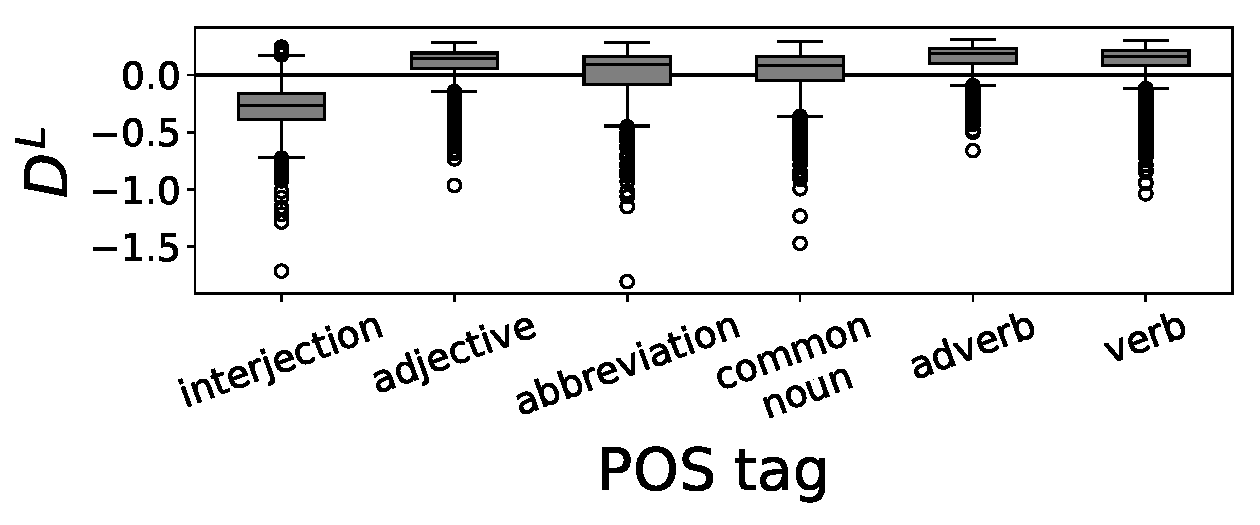
\includegraphics[width=\columnwidth]{figures/pos_DL_distribution.pdf}
\caption{Distribution of mean linguistic dissemination ($D^{L}$) across part of speech groups.}
\label{fig:pos-cd-dist}
% scripts/frequency/plot_pos_DL_distribution.py
\end{figure}

Linguistic dissemination can separate words by grammatical category, as shown in \autoref{fig:pos-cd-dist} where the mean $D^{L}$ values are computed for words across common part-of-speech categories.
Part-of-speech tags were computed over the entire corpus using a Twitter-based tagger~\cite{gimpel2011}, and each word type was assigned the most likely POS tag to provide an approximate distribution of tags over the vocabulary.
Interjections have a lower median $D^{L}$ than other word categories due to the tendency of interjections to occur in limited lexical contexts.
Conversely, verbs have  a higher median $D^{L}$ due to the flexibility of verbs' arguments (e.g., subject and object may both be open-class nouns).

%Examples of growth words with high and low linguistic dissemination are shown in \autoref{tab:predictor-example-words}. 
%High dissemination words include flexible acronyms (\example{aka}) and modifiers that can apply to a variety of contexts (\example{ish}).
%Words with low linguistic dissemination include words that are often used in sentence initial or final position (\example{yikes}).
%, and more topic-specific words (\example{ooc}, \gloss{out of character}). 
%These differences are due in part to the grammatical aspects of linguistic dissemination: for instance, adjectives (\example{ingame}) tend to have higher context diversity than interjections (\example{yeah}). 

%\paragraph{Grammatical aspects of linguistic dissemination} 
%To confirm the grammatical aspects captured by linguistic dissemination, we visualize the distribution of $D^{L}$ values across words grouped by part of speech tags.
%%The grammatical aspects of linguistic linguistic dissemination are confirmed with the distribution of $D^{L}$ across part of speech tags. 
%These tags were obtained automatically from the CMU Twitter Part-of-Speech tagger~\cite{gimpel2011}.\footnote{\url{https://github.com/brendano/ark-tweet-nlp} (Accessed 17 June 2017).}
%As shown in \autoref{fig:pos-cd-dist}, interjections have lower linguistic dissemination, which follows from being restricted to sentence-initial or sentence-final position. 
%In contrast, adjectives and adverbs have high linguistic dissemination because they can appear throughout the sentence, often near open-class words such as nouns and verbs. 
%But while these differences are real and in some cases substantial (one-way ANOVA between part-of-speech groups: $F=822.6, p < 0.0001$), robustness checks in ~\autoref{sec:results-binary-predict} show that the role of linguistic dissemination in explaining word growth goes beyond part-of-speech category.
% ANOVA results: output/tag_vs_DC_ANOVA.tsv
%Some part of speech groups such as proper nouns have lower bigram context diversity than trigram context diversity, which may reflect how proper nouns in English often occur in pairs (e.g. \example{Hillary Clinton}) and have more restricted bigram contexts than trigram contexts.
%interjections tend to have a less diverse trigram context (e.g. \emph{omg} often followed by multiple exclamation points).
%Bigram context diversity also has larger variance in nearly all part of speech categories as compared to trigram context diversity, which demonstrates that short-term dependencies (bigrams) are less predictable than long-term dependencies (trigrams).
%We find that bigram and trigram context diversity are highly collinear ($R=0.91$), and we choose to include only trigram diversity in our experiments. \ian{not sure if this is enough justification}

%we use this metric to approximate the linguistic factors that influence the adoption of a lexical innovation. 
% diversity to find words with an unexpectedly high number of bigram and trigram context counts, we can approximate the semantic diversity of lexical innovations as a proxy for linguistic context to contrast with the social context (dissemination).

%\ian{should we show examples of $C^{2}$ and $C^{3}$ disagreeing? e.g. where a word has high $C^{3}$ and low $C^{2}$.}

%Following prior work in quantifying polysemy~\cite{hamilton2016change}, we use the embeddings computed at each timestep to build a network of related words. We connect two words $w_{i}$ and $w_{j}$ with an edge if $w_{j}$ is one of the $k$-nearest neighbors of $w_{i}$, determined by cosine distance between the embeddings. We set $k=10$ \ian{through experimentation?}. For each word in the network, we then compute the clustering coefficient

\section{Results}
The hypotheses about social and linguistic dissemination are tested under four analyses: correlation against frequency change in growth words; causal inference on probability of word growth; binary prediction of word growth; and survival analysis of decline words.
%We find evidence in support of hypotheses H1, H2 and H2a, such that both social dissemination and context dissemination play an important role in predicting innovation success.

\subsection{Correlational analysis}
\label{subsec:relative-importance}
To test the relative importance of the linguistic and social context on word growth, we correlate these metrics with frequency change ($\Delta_{f_{t}} = f_{t} - f_{t-k}$) across all growth words. 
This replicates the methodology in prior work by \newcite{altmann2011} and \newcite{garley2012}, who analyzed different internet forums.
Focusing on long-term change with $k=12$ (one year) and $k=24$ (two years), 
%we compute the correlation between each covariate at time $t-k$ and the frequency change from $t-k$ to $t$,
we compute the proportion of variance in frequency change explained by the covariates using a relative importance regression~\cite{kruskal1987}.\footnote{Relative importance regression implemented in the \emph{relaimpo} package in R: \url{https://cran.r-project.org/package=relaimpo}}

The results of the regression are shown in \autoref{tab:relative-importance-test}. 
All predictors have relative importance greater than zero, according to a bootstrap method to produce confidence intervals~\cite{tonidandel2009}. 
Frequency is the strongest predictor ($f_{t-12}, f_{t-24}$), because words with low initial frequency often show the most frequency change.
In both short- and long-term prediction, linguistic dissemination ($D^{L}_{t-12}, D^{L}_{t-24}$) has a higher relative importance than each of the social dissemination metrics.
%, indicating the importance of lexical flexibility in predicting word growth. 
The social dissemination metrics have less explanatory power, in comparison with the other predictors and in comparison to the prior results of \newcite{garley2012}, who found $1.5\%$ of variance explained by $D^{U}$ and $1.9\%$ for $D^{T}$ at $k=24$.
Our results were robust to the exclusion of the predictor $D^L$, meaning that a model with only the social dissemination metrics as predictors resulted in a similar proportion of variance explained.
The weakness of social dissemination could be due to the fragmented nature of Reddit, compared to more intra-connected forums. 
Since users and threads are spread across many different subreddits, and users may not visit multiple subreddits, a higher social dissemination for a particular word may not lead to immediate growth.

\begin{table}[t!]
\small
\centering
\begin{tabular}{l r r }
  \toprule
  ~ & \specialcell{Variance \\ explained} & Lower, upper 95\% \\
  \midrule
$f_{t-12}$ & 10.8\% & [10.2\%, 11.5\%]  \\ 
$D^{L}_{t-12}$ & 0.584\% & [0.461\%, 0.777\%]  \\ 
$D^{U}_{t-12}$ & 0.307\% & [0.251\%, 0.398\%] \\ 
$D^{S}_{t-12}$ & 0.120\% & [0.0852\%, 0.191\%] \\ 
$D^{T}_{t-12}$ & 0.246\% & [0.171\%, 0.379\%]  \\[2ex]
$f_{t-24}$ & 21.4\% & [20.4\%, 22.4\%] \\ 
$D^{L}_{t-24}$ & 1.29\% & [1.05\%, 1.64\%] \\ 
$D^{U}_{t-24}$ & 0.400\% & [0.346\%, 0.493\%] \\ 
$D^{S}_{t-24}$ & 0.287\%  & [0.201\%, 0.392\%] \\ 
$D^{T}_{t-24}$ & 0.272\% & [0.226\%, 0.380\%] \\ \bottomrule
% output/results/relative_importance_coefficients_f_DU_DS_DT_DL.tsv
\end{tabular}

\caption{Percent of variance explained in frequency change, computed over all growth words $\set{G}$.
$N=26,880$ for $k=12$, $N=13,440$ for $k=24$.} 
\label{tab:relative-importance-test}
\end{table}

\subsection{Causal analysis}
\label{sec:results-causal}
While correlation can help explain the relationship between dissemination and frequency change, it only addresses the weak version of H2: it does not distinguish the causal impact of linguistic and social dissemination. 
To test the strong version of H2, we turn to a causal analysis, in which the \emph{outcome} is whether a nonstandard word grows or declines, the \emph{treatment} is a single dissemination metric such as linguistic dissemination, and the \emph{covariates} are the remaining dissemination metrics. 
The goal of this analysis is to test the impact of each dissemination metric, while holding the others constant. 

\begin{figure*}
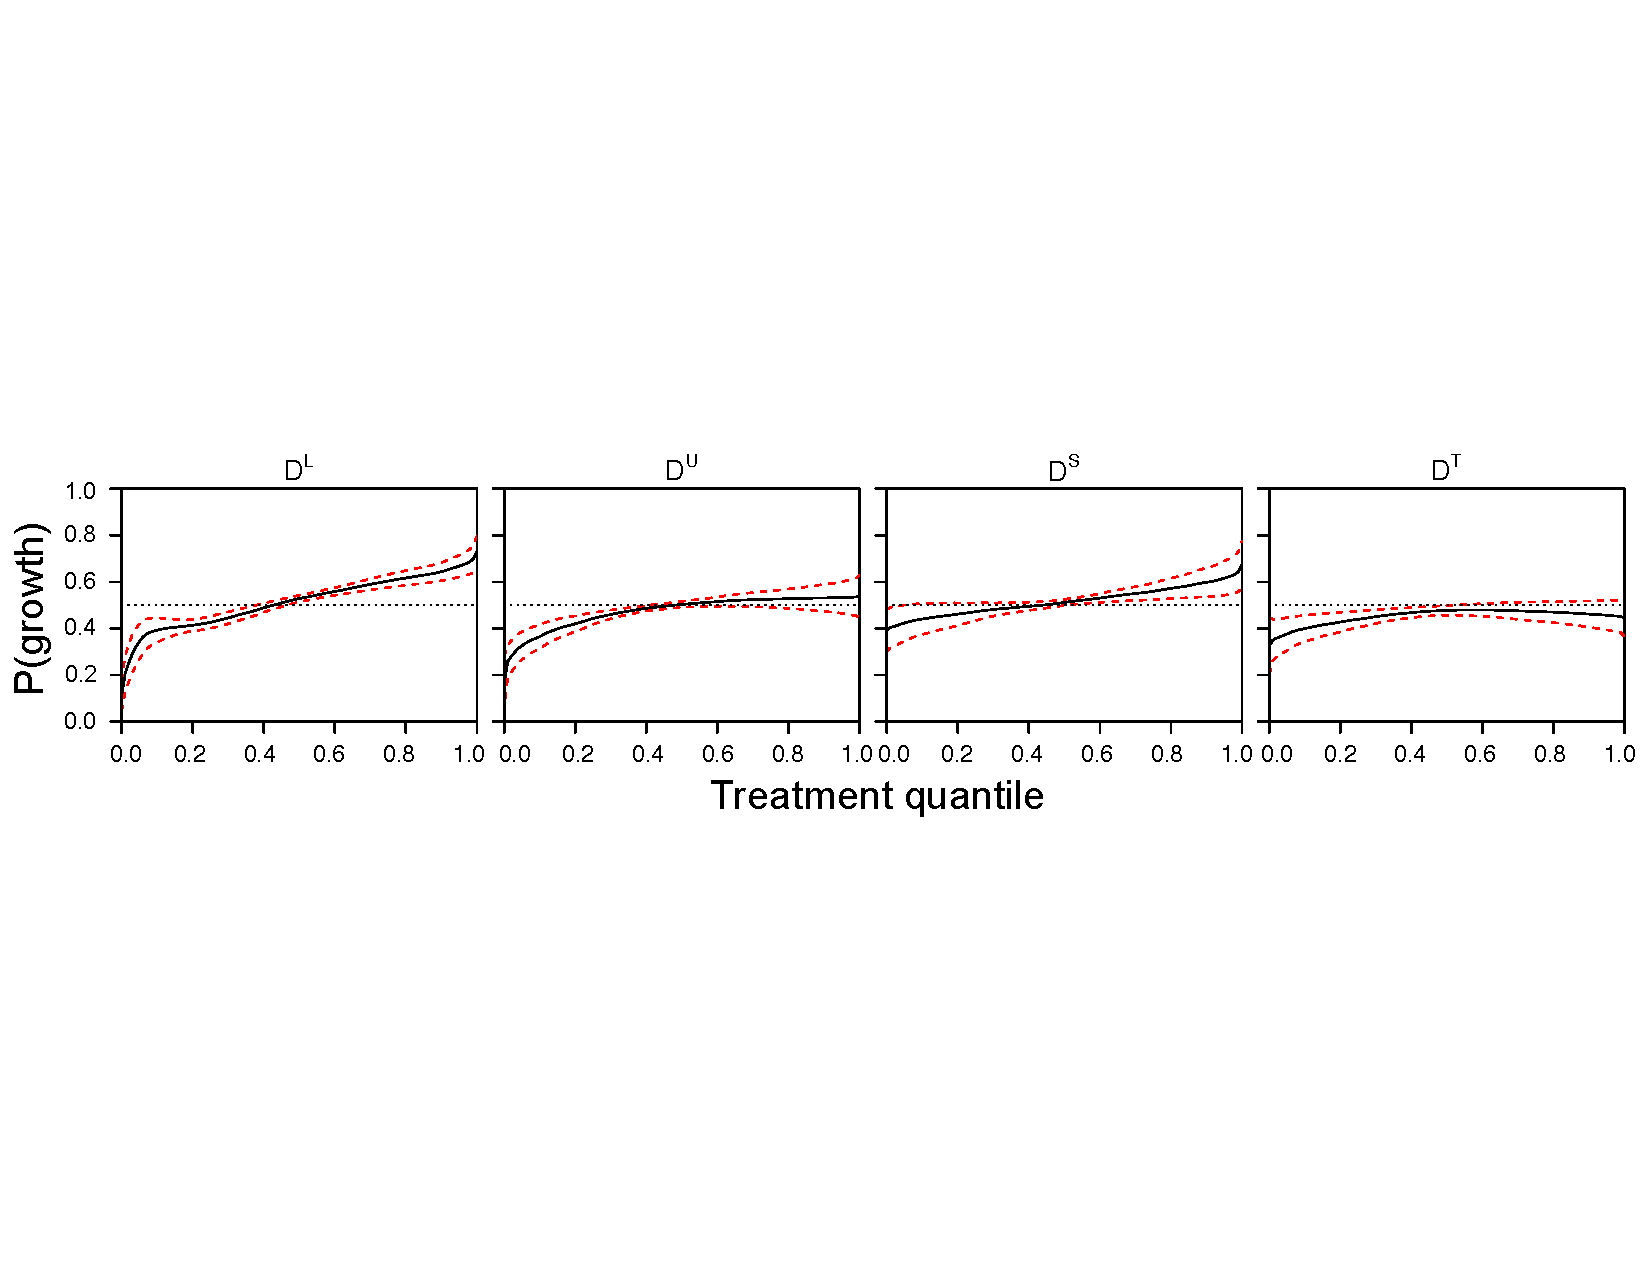
\includegraphics[width=\textwidth]{figures/ADRF_curves_1_12_100_DL,DU,DS,DT.pdf}
% generated with scripts/prediction/plot_average_dose_response_function.R
\caption{Average dose response function for all treatment variables, where outcome is probability of word growth. 95\% confidence intervals plotted in red, chance rate of 50\% marked with dotted black line.}
\label{fig:ADRF_curves}
\end{figure*}

Causal inference typically uses a binary treatment/control distinction~\cite{angrist1996}, but in this case the treatment is continuous. 
We therefore turn to an adapted model known as the \emph{average dose response function} to measure the causal impact of dissemination~\cite{imbens2000}.
To explain the procedure for estimating the average dose response, we adopt the following terminology: $Z$ for treatment variable, $X$ for covariates, $Y$ for outcome.\footnote{Average dose response function implemented in the \emph{causaldrf} package in R: \url{https://cran.r-project.org/package=causaldrf}}
\begin{enumerate}
\setlength{\itemsep}{1pt}
\item A linear model is fit to estimate the treatment from the covariates,
  \begin{equation}
    Z_{i} \mid X_{i} \sim \mathcal{N}(\beta^{\top} X_{i},\sigma^{2}).
  \end{equation}
  The output of this estimation procedure is a vector of weights $\hat{\beta}$ and a variance $\hat{\sigma}^2$. 
\item The generalized propensity score (GPS) $R$ is the likelihood of observing the treatment given the covariates, $P(Z_{i} \mid X_{i})$. It is computed from the parameters estimated in the previous step:
  \begin{equation}
    \hat{R}_i = \frac{1}{\sqrt{2\pi\hat{\sigma}^{2}}} \exp \left(-\frac{(Z_{i} - \hat{\beta}^{\top}X_{i})^{2}}{2\hat{\sigma}^{2}}\right).
  \end{equation}
\item A logistic model is fit to predict the outcome $Y_{i}$ using the treatment $Z_{i}$ and the GPS $\hat{R}_i$:
  \begin{equation}
    \hat{Y}_{i} = \text{Logistic}(\hat{\alpha}_{0} + \hat{\alpha}_{1}Z_{i} + \hat{\alpha}_{2}\hat{R}_i).
  \end{equation}
  This involves estimating the parameters $\{\hat{\alpha}_0, \hat{\alpha}_1, \hat{\alpha}_2.\}$
By incorporating the generalized propensity score $\hat{R}_i$ into this predictive model over the outcome, it is possible to isolate the causal effect of the treatment from the other covariates~\citep{hirano2004}.
\item The range of treatments is divided into levels (quantiles). The \emph{average dose response} for a given treatment level $s_{z}$ is the mean estimated outcome for all instances at that treatment level,
\begin{equation}
\hat{\mu}(s_{z}) = \frac{1}{| s_{z} |} \sum_{z_{i} \in s_{z}} \hat{Y}_{i}.
\end{equation}
The average dose response function is then plotted for all treatment levels.
\end{enumerate}

Each dissemination metric is considered separately as a treatment. 
We consider all other dissemination metrics and frequency as covariates: e.g., for treatment variable $D^{L}$, the covariates are set to $[f,D^{U},D^{S},D^{T}]$.
We bootstrap the above process 100 times with different samples to produce confidence intervals.
To balance the outcome classes, we sample an equal number of growth and decline words for each bootstrap iteration.

The average dose response function curves in \autoref{fig:ADRF_curves} show that linguistic dissemination ($D^{L}$) produces the most dramatic increase in word growth probability.
For linguistic dissemination, the lowest treatment quantile (0\%-10\%) yields a growth probability below 40\% (significantly less than chance), as compared to the highest treatment quantile (90-100\%), which yields a growth probability nearly at 70\% (significantly greater than chance). 
This supports the strong form of H2, which states that linguistic dissemination is predictive of growth, even after controlling for the frequency and the other dissemination metrics. 
Subreddit dissemination also shows a mild causal effect on word growth, up to 60\% in the highest treatment quantile.
The other social dissemination metrics prove to have less effect on word growth.

\subsection{Predictive analysis}
\label{sec:results-binary-predict}
We now turn to prediction to determine the utility of linguistic and social dissemination: using the first $k$ months of data, can we predict whether a word will grow or decline in popularity?
This is similar to previous work in predicting the success of lexical innovations~\cite{kooti2012predicting}, but our goal is to compare the relative predictive power of various dissemination metrics, rather than to maximize accuracy.

\begin{figure}
\centering
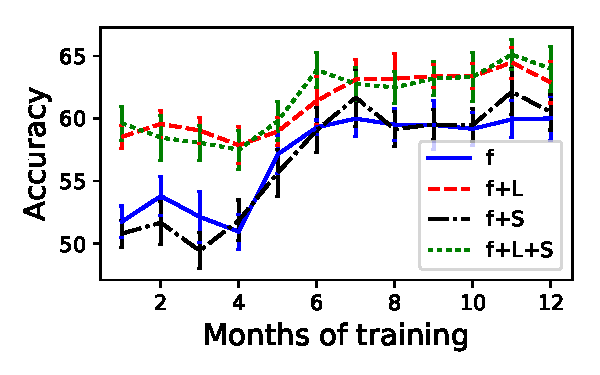
\includegraphics[width=\columnwidth]{figures/success_1_12_window_lines.pdf}
\caption{Prediction accuracy for different feature sets using $k={1...12}$ months of training data. $f$ indicates frequency-only, $f+L$ frequency plus linguistic dissemination, $f+S$ frequency plus social dissemination, $f+L+S$ all features.}
\label{fig:success_accuracy}
% scripts/prediction/plot_growth_k_month_window_lines.py
\end{figure}

We use logistic regression with 10-fold cross-validation over four different feature sets: frequency-only (\model{f}), frequency plus linguistic dissemination (\model{f+L}), frequency plus social dissemination (\model{f+S}) and all features (\model{f+L+S}).
Each fold is balanced for classes so that the baseline accuracy is 50\%.
\autoref{fig:success_accuracy} shows that linguistic dissemination provides more predictive power than social dissemination: the accuracy is consistently higher for the models with linguistic dissemination than for the frequency-only and social dissemination models.
The accuracies converge as the training data size increases, which suggests that frequency is a useful predictor if provided sufficient historical trajectory.

%% ADRF prediction

%\begin{figure}[t!]
%\centering
%\includegraphics[width=0.7\columnwidth]{figures/ADRF_accuracy_1_12_DL,DS,DU,DT,f.pdf}
%% generated with scripts/prediction/plot_average_dose_response_function_accuracy.R
%\caption{Accuracy on predicting success from fail words using different treatment models (10-fold cross-validation).}
%\label{fig:ADRF_accuracy}
%\end{figure}

%We further investigate the predictive power of the different dissemination metrics as follows: using the parameters estimated for the dose response function, what is the accuracy of predicting lexical success?

%For each treatment variable, a logistic regression model is parameterized using the mean of the parameters computed in (3) and used to predict success versus failure using the first $k=12$ months of data.
%The baseline model is a frequency-only logistic regression in which the mean frequency over the first $k=12$ months of data is used to predict success versus failure.
%This process is conducted using 10-fold cross-validation and the AUC accuracy is measured to compare the predictive power of different treatments.
%The results in~\autoref{fig:ADRF_accuracy} demonstrate that the model using linguistic dissemination (DL) performs the best (66\%), followed by the model with user dissemination (DU; 60\%).
%This aligns with the results from the ADRF curves, which showed a significant difference in probability of success between the low- and high-treatment conditions.

\begin{figure}
\centering
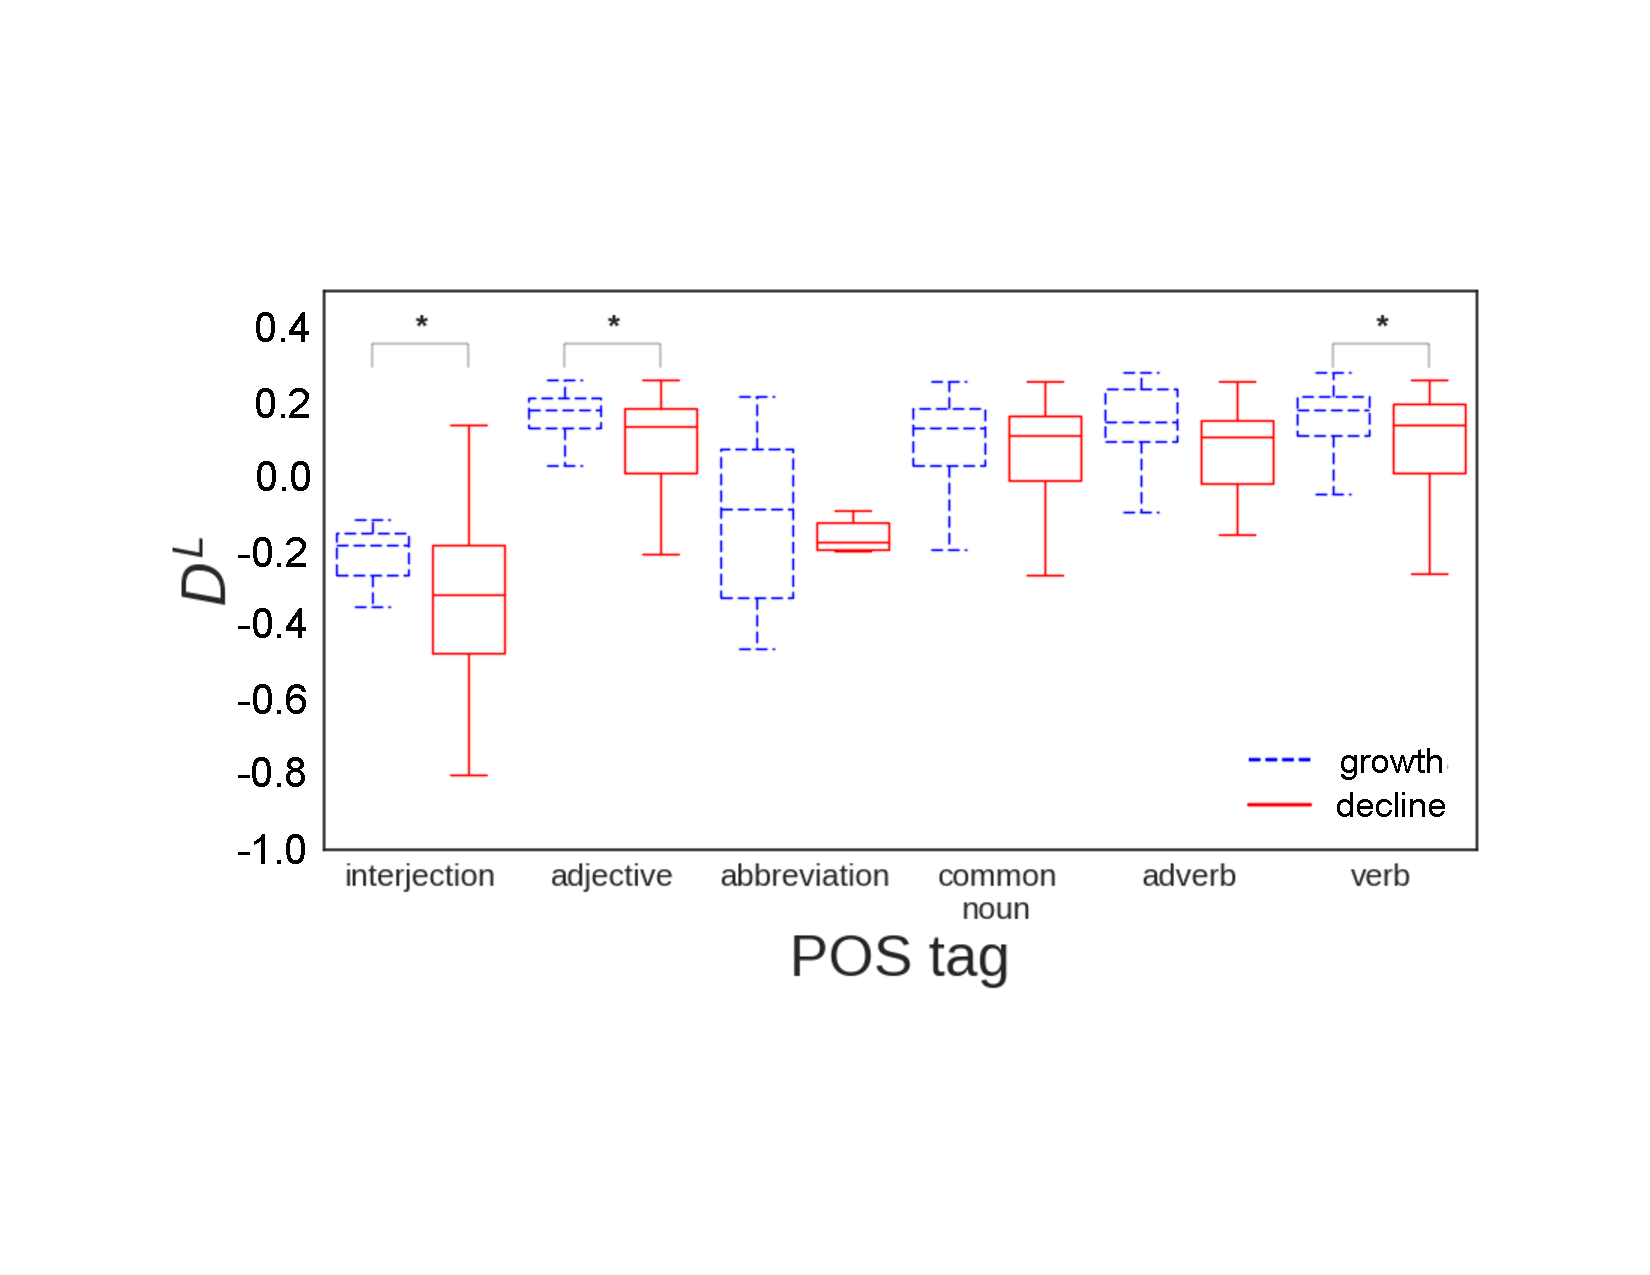
\includegraphics[width=\columnwidth]{figures/growth_vs_decline_matched_pos_DL_distribution_1_12.pdf}
% generated with scripts/frequency/plot_success_vs_failure_pos_DL_distribution.sh
\caption{Distribution of $D^{L}$ values across growth and decline words, grouped by part of speech tag. 
* indicates $p<0.05$ in one-tailed t-test between growth and decline $D^{L}$ values.}
\label{fig:success_vs_failure_pos_DL_distribution}
\end{figure}

\paragraph{Part-of-speech robustness check}

Considering the uneven distribution of linguistic dissemination across part-of-speech groups (\autoref{fig:pos-cd-dist}), the prediction results may be explained by an imbalance of word categories between the growth and decline words.
This issue is addressed through two robustness checks: within-group comparison and prediction.

First, we compare the distribution of linguistic dissemination values between growth and decline words, grouped by the most common POS tags (computed in \autoref{sec:linguistic_dissemination}).
Each decline word is matched with a growth word based on similar mean frequency in the first $k=12$ months, and their mean linguistic dissemination values during that time period are compared, grouped within POS tag groups.
The differences in~\autoref{fig:success_vs_failure_pos_DL_distribution} show that across all POS tags, the growth words show a tendency toward higher linguistic dissemination with significant ($p<0.05$) differences in the interjections and verbs.

%To address this possibility, the POS tags (computed in \autoref{sec:linguistic_dissemination}) are added as additional features to the binary prediction task.
Next, we add POS tags as additional features to the frequency-only model in the binary prediction task.
The accuracy of a predictive model with access to frequency and POS features at ${k=1}$ is 54.8\%, which is substantially lower than the accuracy of the model with frequency and linguistic dissemination (cf. \autoref{fig:success_accuracy}).\footnote{Higher $k$ values yield similar results.}
Thus, linguistic dissemination thus contributes predictive power beyond what is contributed by part-of-speech alone.
% scripts/prediction/predict_growth_POS_tag.py

\subsection{Survival analysis}
\label{sec:results-survival}
Having investigated what separates growth from decline, we now focus on the factors that precede a decline word's ``death'' phase~\cite{drouin2009}.
%We now focus on the factors that precede a word's decline phase, which can be viewed as the beginning of ``word death''~\cite{drouin2009} for many of these terms --- though some may emerge again later. 
%We use the decline words as ``uncensored'' data, words with an observed death date, and the growth words as ``censored'' data, words with an unobserved death date.
%The distribution of survivors is shown in Figure \ref{fig:split_point_dist}, which shows that most of the decline words begin to decline before the year mark ($t=12$). 
%\begin{figure}[t!]
%\centering
%\includegraphics[width=\columnwidth]{figures/split_point_survivor_curve.pdf}
%\caption{Survival curve of all decline and growth words.}
%%\caption{Survival curve of all failure and success innovations, dotted line indicates number of success (i.e. non-death) innovations.}
%\label{fig:split_point_dist}
%\end{figure}
Predicting the time until a word's decline can be framed as survival analysis~\cite{klein2005}, in which a word is said to ``survive'' until the beginning of its decline phase at split point $\hat{t}$. 
In the Cox proportional hazards model~\cite{david1972}, the hazard of death $\lambda$ at each time $t$ is modeled as a linear function of a vector of predictors,
\begin{equation}
  \lambda_i(t)  = \lambda_0(t) \exp (\mathbf{\beta} \cdot \mathbf{x}_i),
\end{equation}
where $\mathbf{x}_i$ is the vector of predictors for word $i$, and $\mathbf{\beta}$ is the vector of coefficients. Each cell $x_{i,j}$ is set to the mean value of predictor $j$ for word $i$ over the training period $t=\{1 ... k\}$ where $k=3$.

For words which begin to decline in popularity in our dataset, we treat the point of decline as the ``death'' date. The remaining words are viewed as \emph{censored} instances: they may begin to decline in popularity at some point in the future, but this time is outside our frame of observation.
We use frequency, social dissemination and linguistic dissemination as predictors in a Cox regression model.\footnote{Cox regression implemented in the \emph{lifelines} package in Python: \url{https://lifelines.readthedocs.io/en/latest/}.}

\begin{table}[t!]
\small
\centering
\begin{tabular}{l r r r r}
\toprule
  Predictor & $\beta$ & std. error & $Z$ & $p$ \\ \midrule
% old results
%$f$ & -0.208 & 0.0399 & -5.21 & *** \\ 
%$D^{L}$ & -0.310 & 0.0346 & -8.96 & *** \\ 
%$D^{U}$ & -0.0845 & 0.0583 & -1.45 & ~ \\ 
%$D^{S}$ & -0.127 & 0.0596 & -2.13 & * \\ 
%$D^{T}$ & 0.0819 & 0.0727 & 1.13 & ~ \\ 
$\var{f}$ & -0.207 & 0.0492 & -4.21 & *** \\ 
$\var{D^{L}}$ & -0.330 & 0.0385 & -8.56 & *** \\ 
$\var{D^{U}}$ & 0.0053 & 0.0518 & 0.102 & ~ \\ 
$\var{D^{S}}$ & -0.156 & 0.0807 & -1.928 & ~ \\ 
  $\var{D^{T}}$ & 0.0825 & 0.0662 & 1.25 & ~ \\
  \bottomrule
\end{tabular}
\caption{Cox regression results for predicting word death with all predictors (\model{f+L+S}) averaged over first $k=3$ months.
%Concordance=0.623, where 0.50 represents random chance. 
*** indicates $p<0.001$, otherwise $p>0.05$.}
%\ian{results with $t={0:3}$}}
\label{tab:cox_regression_growth_decline_up_to_3}
% prediction/survival_analysis_python.ipynb#Limited-time-range
% prediction/survival_analysis_tests.py
% output/cox_regression_first_3.txt
\end{table}

The estimated coefficients from the regression are shown in \autoref{tab:cox_regression_growth_decline_up_to_3}.
We find 
%a weak positive coefficient for bigram context diversity and 
a negative coefficient for linguistic dissemination ($\beta=-0.330, p<0.001$), which mirrors the results from \autoref{sec:results-causal}: 
%higher $C^{2}$ and 
higher $D^{L}$ indicates a lower hazard of word death, and therefore a higher likelihood of survival.
%We also find weak negative coefficients ($p>0.05$) for user and subreddit dissemination, suggesting 
We also find that higher subreddit dissemination has a weak but insignificant correlation with a lower likelihood of word death ($\beta=-0.156, p>0.05$).
Both of these results lend additional support to the strong form of the hypothesis H2.
%Thread dissemination pointed in the opposite direction 
%(consistent with the finding from ~\newcite{altmann2011}), (cf. Fig 4 in Altmann et al 2011)
%and user dissemination had no significant effect. 

%\begin{table}[t!]
%\small
%\centering
%\begin{tabular}{l l l l l}
  \toprule
Model & Deviance & d.f. & $\chi^{2}$ & $p$-value \\ \midrule
Null & 4383 & 0 & ~ & ~ \\ 
\model{f} & 4375 & 1 & 16.19 & *** \\ 
\model{f+S} & 4370 & 4 & 27.24 & *** \\ 
\model{f+L} & 4337 & 2 & 93.32 & *** \\ 
\model{f+L+S} & 4331 & 5 & 103.8 & *** \\ 
\bottomrule
%output/cox_regression_deviance_output.txt
\end{tabular}
%\caption{Deviance values for relevant survival models.
%%survival model that uses frequency ($f$), frequency plus dissemination ($f+S$), frequency plus context diversity ($f+L$), and frequency plus context diversity plus dissemination ($f+L+S$). 
%$\chi^{2}$ values based on the likelihood ratio test comparing each model to the null model. 
%Lower deviance indicates better model fit.
%*** indicates $p<0.001$.}
%\label{tab:cox_regression_deviance}
%%survival_analysis_R.ipynb#Survival-analysis-separate-factors
%\end{table}

%The role of each factor is tested by comparing the goodness-of-fit for Cox regression models using different feature sets: frequency (\model{f}), frequency plus linguistic dissemination (\model{f+L}), frequency plus social dissemination (\model{f+S}) and all factors (\model{f+L+S}). 
%The results in \autoref{tab:cox_regression_deviance} demonstrate that the model with dissemination and the model with linguistic diversity each have significantly better-than-null fits (lower deviance than null model).
%However, the all-factor model (\model{f+L+S}) does not have a significantly lower deviance than the linguistic dissemination model (\model{f+L}) ($\chi^{2}=4.6, p=0.80$), therefore adding social dissemination does not significantly improve the model fit. 
%This points to the especially important role of linguistic dissemination in predicting the word growth, as compared with social dissemination.

The predictive accuracy of survival analysis can be quantified by a \emph{concordance score}. A score of 1.0 on heldout data indicates that the model perfectly predicts the order of death times; a score of 0.5 indicates that the predictions are no better than a chance ordering. We perform 10-fold cross-validation of the survival analysis model, and plot the results in \autoref{fig:cox_regression_concordance_scores}.
%To compare the predictive performance of the separate Cox models, we compute their concordance scores using 10-fold cross-validation.\footnote{The concordance score represents the accuracy of predicting the order of death times: a score of 0.5 implies a random order of death times, and a score of 1.0 implies a perfect order of death times.}
%As shown in \autoref{fig:cox_regression_concordance_scores}, the model incorporating
The model with access to linguistic dissemination (\model{f+L}) consistently achieves higher concordance than the baseline frequency-only model (\model{f}), 
%according to Welch's t-test 
($t=4.29, p<0.001$), and the model with all predictors \model{f+L+S} significantly outperforms the model with access only to frequency and social dissemination \model{f+S} ($t=4.64, p<0.001$).
The result is reinforced by testing the goodness-of-fit for each model with model \emph{deviance}, or difference from the null model. 
The \model{f+L} model has lower deviance, i.e. better fit, than the null model ($\chi^{2}=93.3, p < 0.01$), and the \model{f+L+S} does not have a significantly lower deviance than the \model{f+L} model ($\chi^{2}=4.6, p=0.80$), suggesting that adding social dissemination does not significantly improve model fit.

% output/concordance_score_feature_set_comparison_tests.tsv
\begin{figure}[t!]
\centering
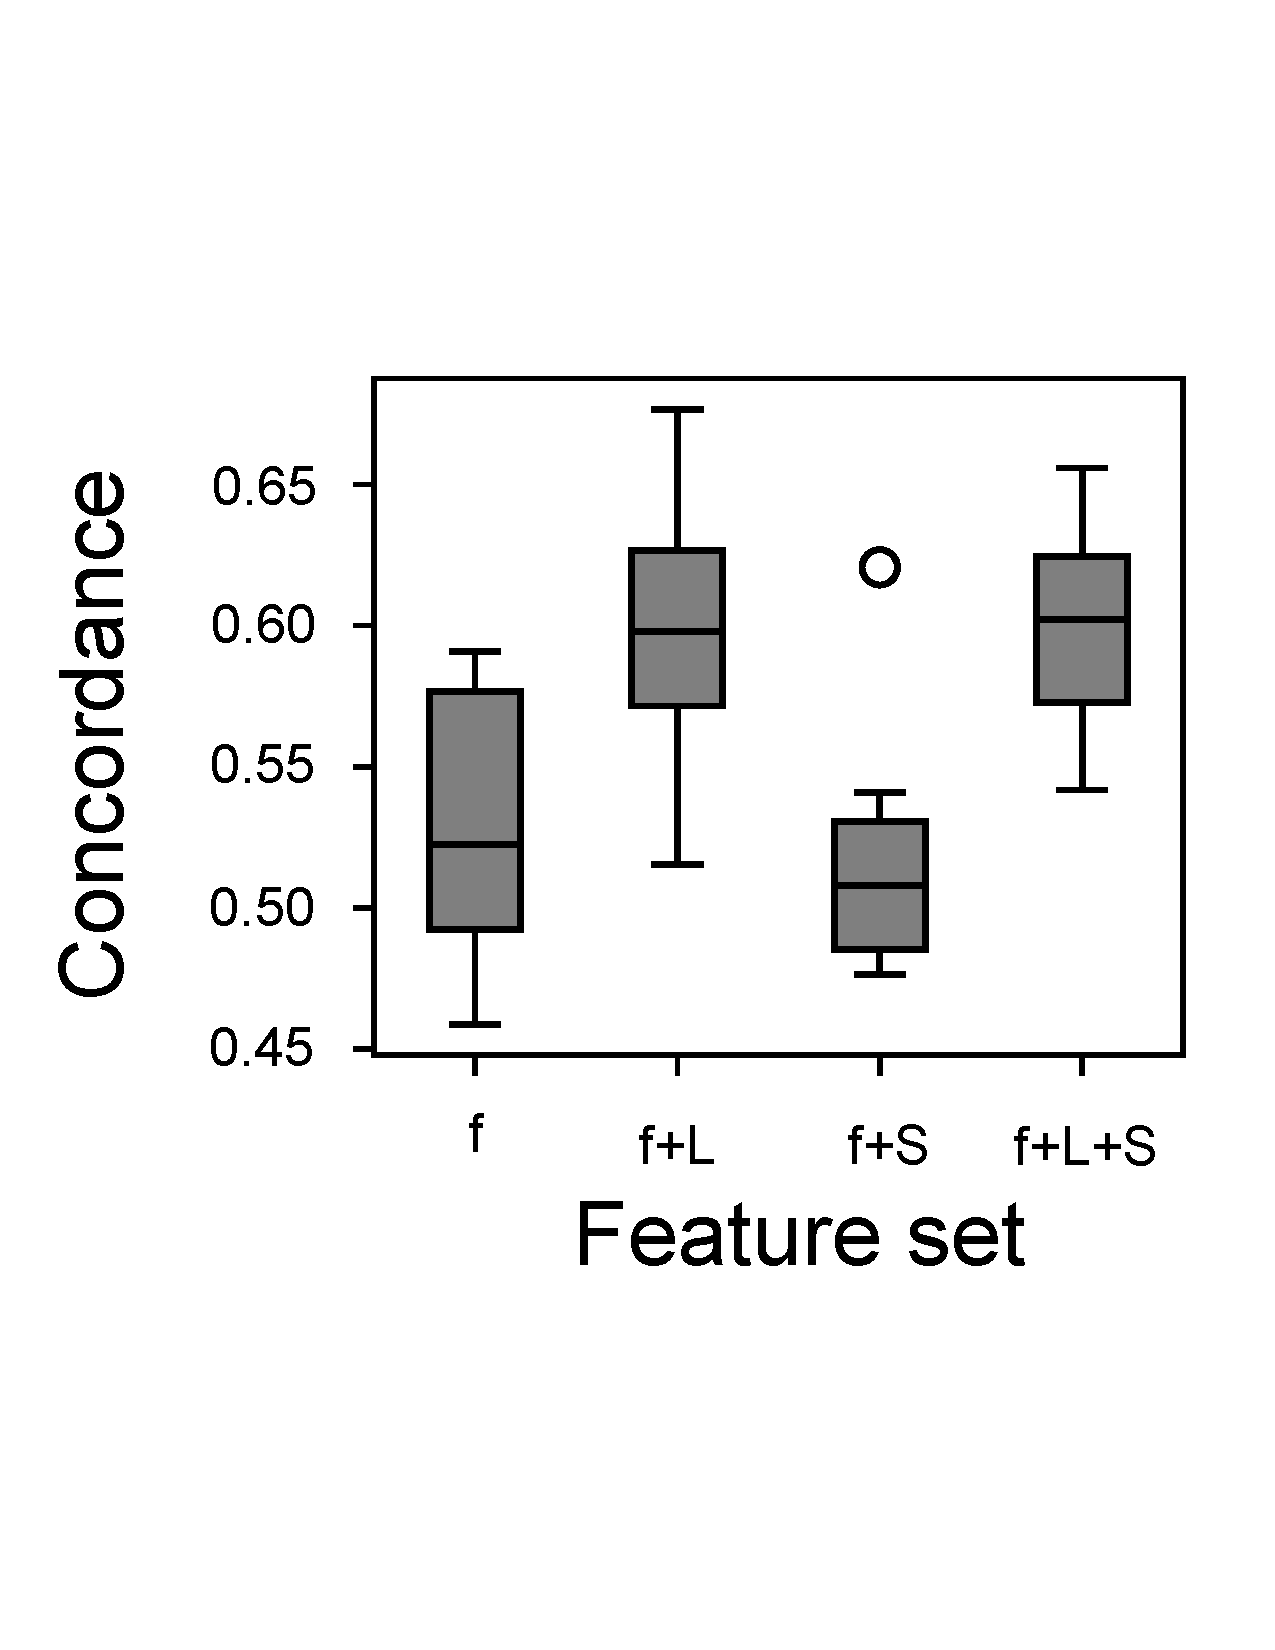
\includegraphics[width=0.8\columnwidth]{figures/survival_concordance_score_distribution.pdf}
\caption{Distribution of concordance scores (10-fold cross-validation) of the Cox regression models across feature sets.}
\label{fig:cox_regression_concordance_scores}
% prediction/plot_concordance_scores.py
\end{figure}



%%%%%%%%%%%%%%%%%%%%%%%%%%%% OLD STUFF

%We therefore test the relative predictive power of the different dissemination metrics with two tests: (1) causal inference and (2) binary prediction of success versus failure.

%\begin{figure}[t!]
%\centering
%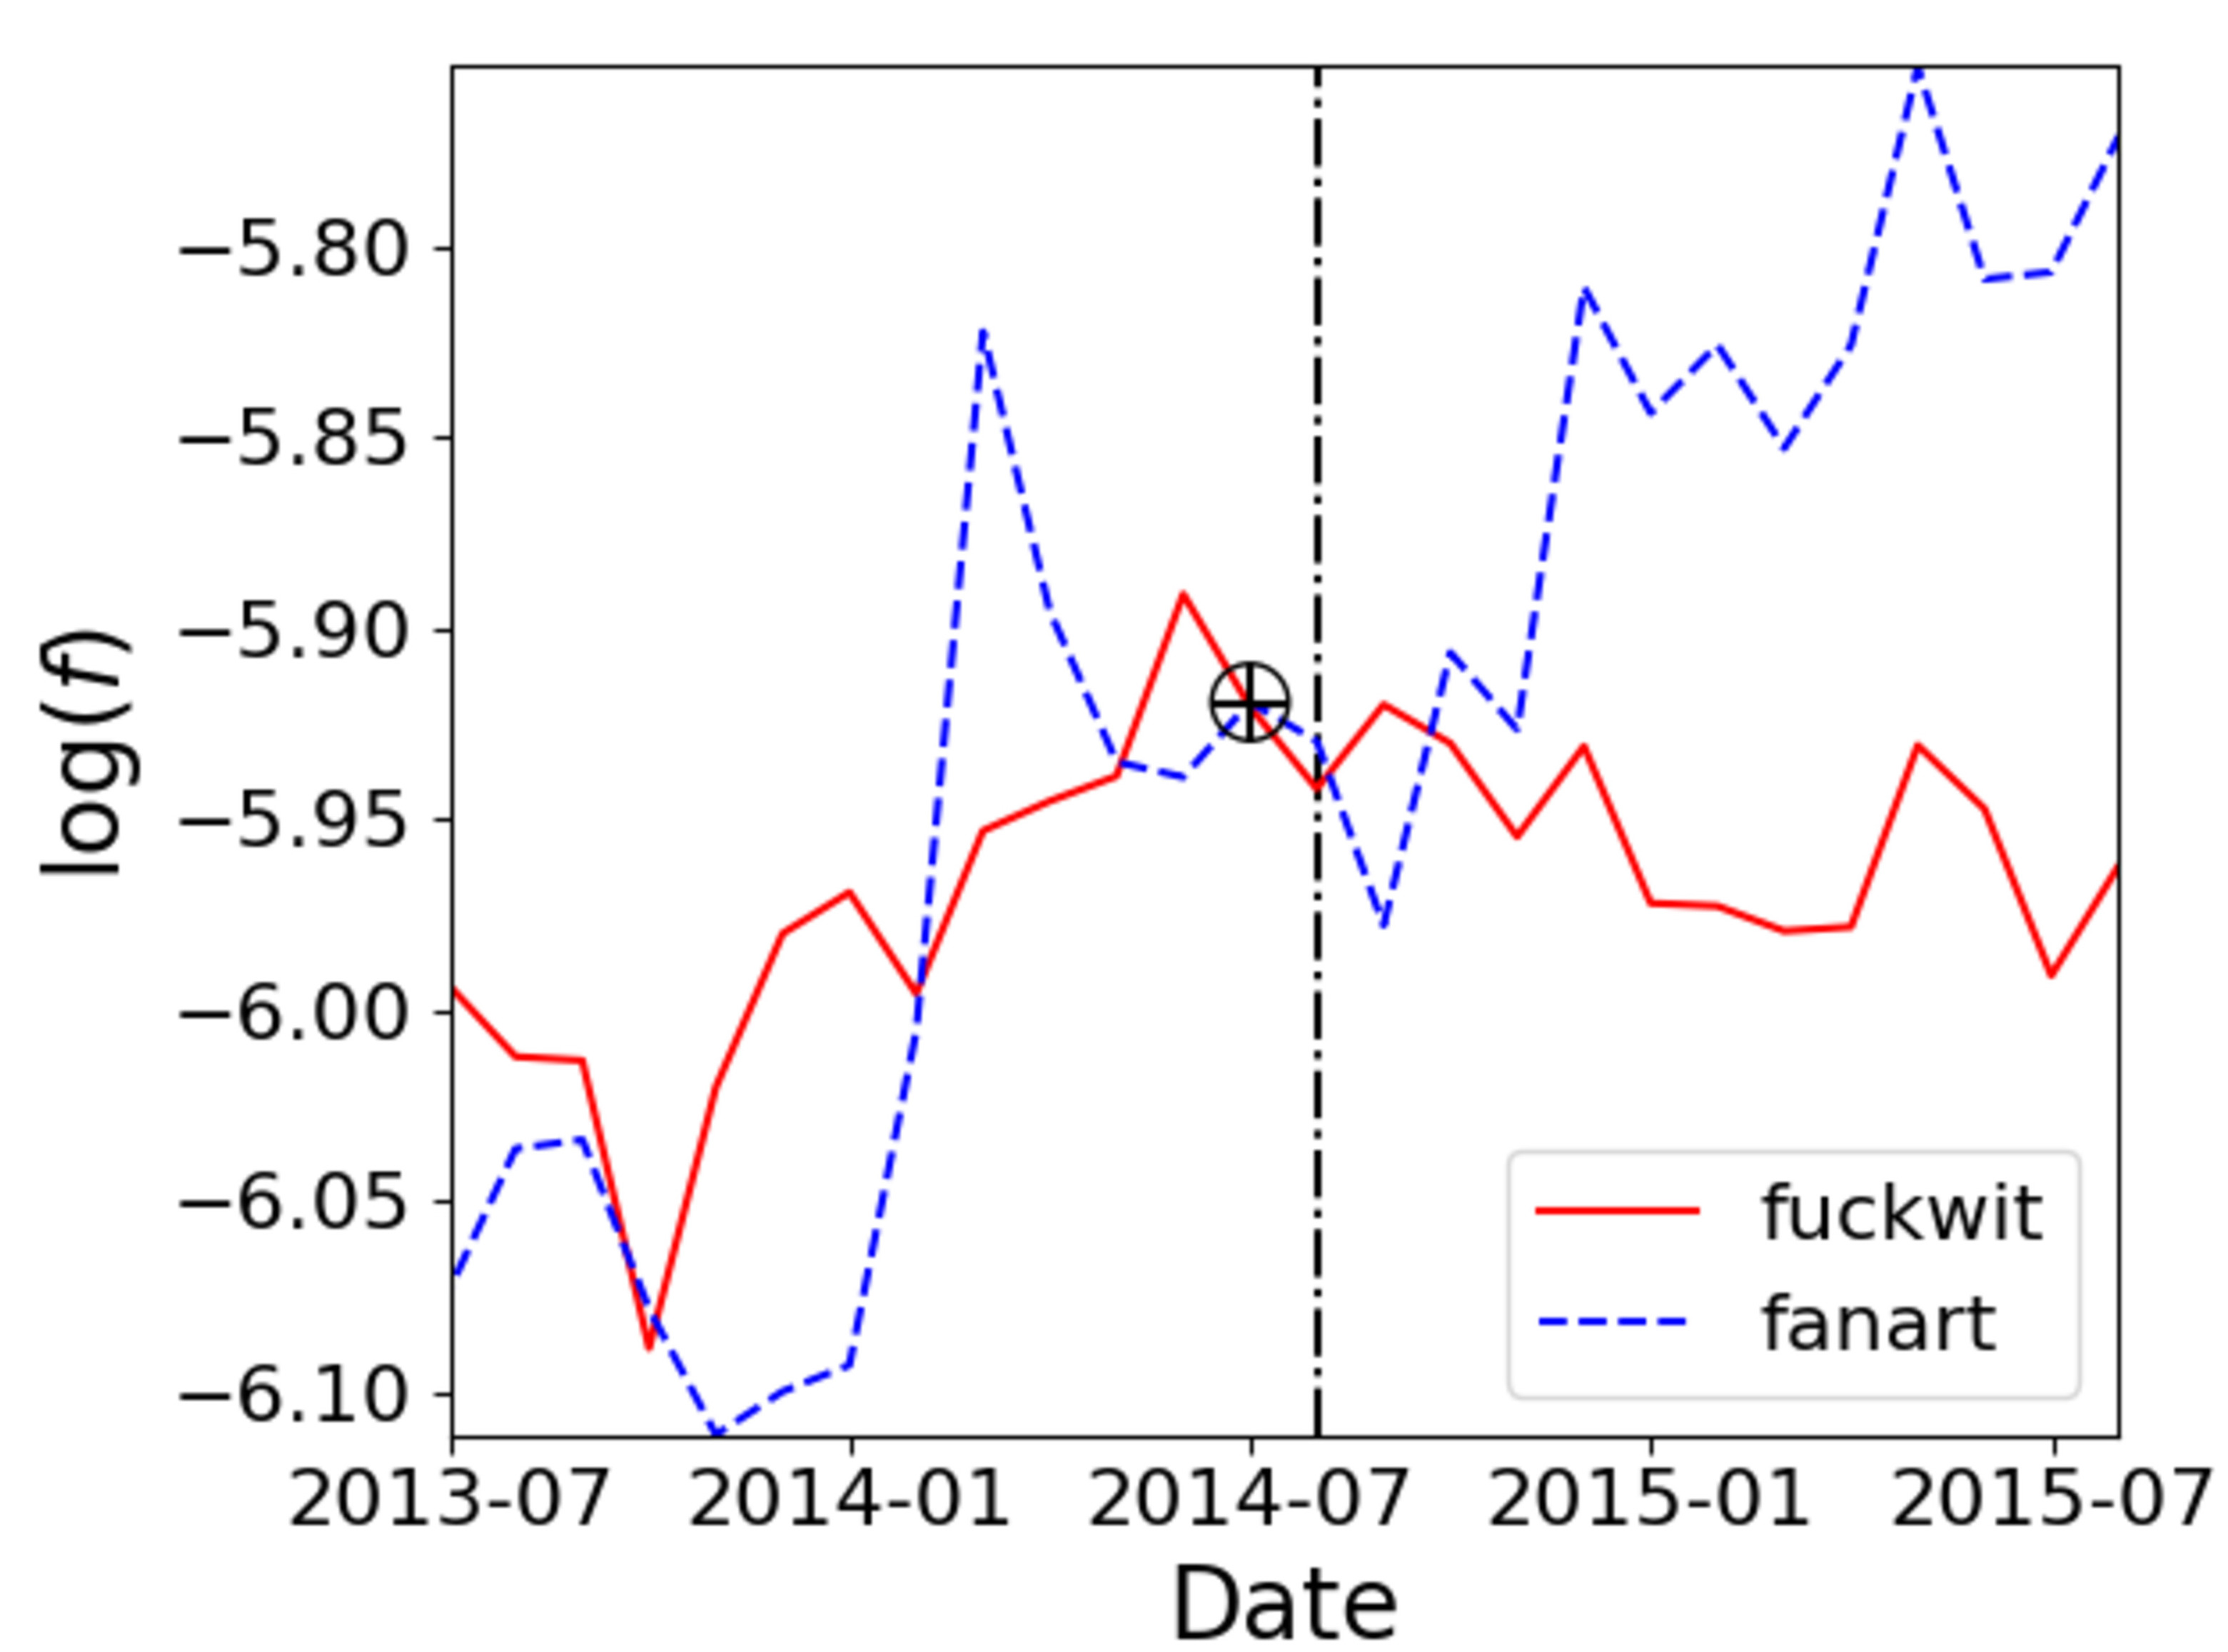
\includegraphics[width=1.0\columnwidth]{figures/match_time_series_example.png}
%\caption{Example failed innovation \example{fuckwit} (\gloss{idiot}) with matched successful innovation \example{fanart}, on $k=1$ month of frequency data.
%  Split point $\hat{t}$ marked at vertical line, match point $\hat{t}-k$ marked with $\bigoplus$.
%  %Vertical lines indicate split point $s$ and prior match points $s-1$.
%}
%\label{fig:growth_decline_match_example}
%\end{figure}
%
%This analysis is based on a prediction task, differentiating successful innovations from a matched failed innovation, using $k$ months of training data.
%Each of the failed innovations $w_{i}$ is matched with a successful innovation $w_{j}$, based on frequency $f$ from $k$ months before the decline phase beginning at split point $\hat{t}$ for $w_i$.
%We optimize the matching by grouping the failed innovation by split point $\hat{t}$ and performing optimal matching within each group~\cite{greevy2004}.\footnote{We use the \textit{optmatch} package for optimal matching within each split point group: \url{https://www.r-pkg.org/pkg/optmatch}.}
%For each split point $\hat{t}$, we gather all failed innovation with the split point into set $\set{F}_{\hat{t}}$ of size $N_{\hat{t}}$ and use optimal matching (without replacement) to find the set of matched success innovations $\hat{M}_{\hat{t}}$ with the best fit.
%The matching procedure attempts to minimize the Mahalanobis distance $D_{m}$ between matched word pairs as follows:
%\begin{align}
%\label{eq:optimal_match}
%%\hat{M}_{\hat{t}} =
%\min_{\set{M}_{\hat{t}}}
%& \quad \sum_{(w_{i}, w_j) \in \set{M}_{\hat{t}}}
%D_{m}(f_{\hat{t}-k:\hat{t}}^{(w_{i})}, f_{\hat{t}-k:\hat{t}}^{(w_{j})})\\
%s.t. & \quad \set{M}_{\hat{t}} \in \textsf{matchings}(\set{G}, \set{F}_{\hat{t}}),
%\end{align}
%where $\textsf{matchings}(\set{G}, \set{F}_{\hat{t}})$ is set of possible matchings between the successful innovations $\set{G}$ and the failed innovations $\set{F}_{\hat{t}}$. 
%An example match is shown in \autoref{fig:growth_decline_match_example}, where the failed innovation \example{fuckwit} is matched with successful innovation \example{fanart} at $\hat{t}-k$, with $k=1$. 
%
%For each matched pair $(w_i, w_j)$ (success, failure), we include $w_i$ with label $y=1$, and $w_j$ with label $y=0$. 
%By design, the resulting dataset will have balanced labels, and equal aggregate frequency across classes at each $\hat{t}$. 
%We then train a logistic regression classifier to predict $y$ (based on $k$ months of data before $\hat{t}$), using the same predictors as in the correlation analysis: frequency, social dissemination and context dissemination. 
%We compare the following sub-sets of the predictors: frequency-only (\model{f}), frequency plus context dissemination (\model{f+L}), frequency plus social dissemination (\model{f+S}) and all features (\model{f+L+S}). 
%To address uncertainty in matching, we bootstrap sample from the failed innovations $\set{F}$ with replacement $B=100$ times. 
%Within each bootstrap sample, we use the matching procedure in \autoref{eq:optimal_match} to construct a dataset and report the 10-fold cross-validated accuracy. 
%
%\begin{figure}[t!]
%\includegraphics[width=\columnwidth]{figures/bootstrap_matched_success_failure_k0_non_differenced_accuracy_10fold.png}
%\caption{Binary prediction accuracy for whether a word will succeed or fail. 
%Prediction performed with logistic regression over 100 bootstrap matching iterations with 10-fold cross-validation in each iteration.}
%% with leave-two-out cross-validation in each iteration.}
%\label{fig:success_failure_prediction_accuracy}
%\end{figure}
%
%\begin{table}[t!]
%\small
%\centering
%\begin{tabular}{l r r r r}
\toprule
  Predictor & \multicolumn{1}{l}{$\mu_{\beta}$} & \multicolumn{1}{l}{$\sigma_{\beta}$} & \multicolumn{1}{l}{$t$} & \multicolumn{1}{l}{$p$} \\ \midrule
const & -0.4935 & 0.3223 & -1.531 & ~ \\
$\var{f}$ & 0.4393 & 0.0651 & 6.748 & *** \\
$\var{D^{C}}$ & 3.824 & 0.3907 & 9.786 & *** \\
$\var{D^{U}}$ & 3.287 & 0.6079 & 5.407 & *** \\
$\var{D^{S}}$ & 1.940 & 0.3784 & 5.127 & *** \\
$\var{D^{T}}$ & -0.7693 & 0.5997 & -1.283 & ~ \\
\bottomrule
\end{tabular}

%\caption{Logistic regression coefficients to predict word success for $k=1$ months of prior data, using the full model (\model{f+L+S}).
%Predictor mean $\mu_{\beta}$, standard error $\sigma_{\beta}$ and $t$ values computed from the sample of $\beta$ coefficients over 100 bootstrap iterations.
%*** indicates $p<0.001$, otherwise $p>0.05$.}
%% output/bootstrap_matched_success_failure_k0_non_differenced_coefficients_10fold_average.tsv
%\label{tab:logit_growth_growth_decline}
%\end{table}
%
%Using $k=1$ as our base case (predicting success from failure using only one month of data prior to the split point), we find that context dissemination and social dissemination both contribute to the likelihood of word success.
%The accuracies in \autoref{fig:success_failure_prediction_accuracy} demonstrate that the combination of context dissemination and social dissemination provides the most information on predicting success from failure. 
%In the full model, the coefficients for $D^C$ are consistently positive (see \autoref{tab:logit_growth_growth_decline}), providing support for hypothesis H2 --- higher context dissemination makes success more likely. 
%The situation for the social dissemination predictors is more complex. 
%$D^S$ and $D^U$ have positive coefficients, but the coefficient for $D^T$ (thread dissemination) is negative and insignificant.
%This contrasts with the findings on $D^{T}$ from~\newcite{altmann2011}, which suggests that on Reddit the dissemination of a word among threads is less important than dissemination among users, as compared to Usenet where thread and user dissemination are comparable.
%%\vspace{-10pt}
%%This may speak to the interactions among users and sub-communities on Reddit, such that a word that reaches a critical mass of users and subreddits is more likely to succeed (more connections among users and among subreddits), as compared to a word that is disseminated across threads (fewer connections among threads).
%%\jacob{I don't understand this explanation}
%
%%In the binary classification task, we find evidence for both hypotheses 1 and 2, because a higher context dissemination and a higher social dissemination contribute to the likelihood of success.
%
%\begin{figure}[t!]
%\centering
%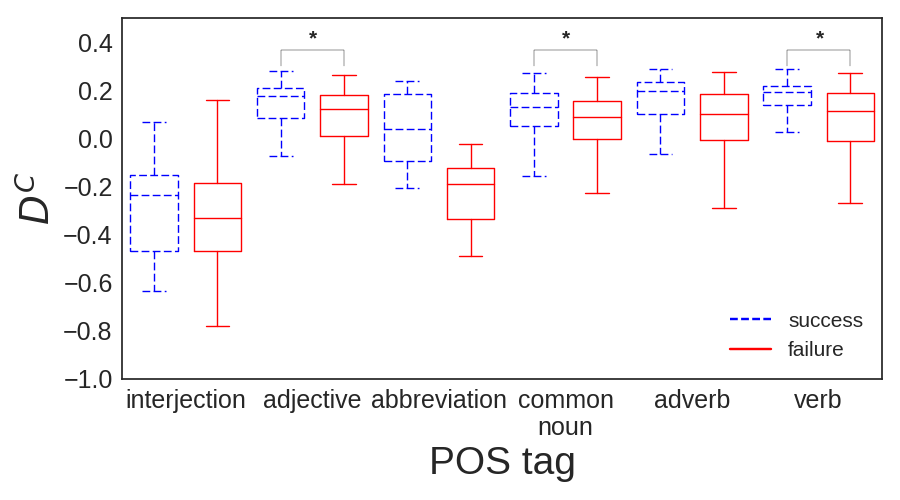
\includegraphics[width=\columnwidth]{figures/success_vs_failure_matched_pos_C3_distribution.png}
%\caption{Distribution of $D^{L}$ values across successful and failed innovation, grouped by part of speech tag. 
%* indicates $p<0.05$ in one-tailed t-test between successful and failed $D^{L}$ values.}
%\label{fig:success_vs_failure_pos_C3_distribution}
%\end{figure}
%
%\paragraph{Robustness checks}
%We perform this same classification task for a range of history lengths, $k \in \{2 ... 8\}$, and find similar accuracy results across the feature sets: \model{f+L+S} outperforms \model{f+L} and \model{f+S}, which outperform \model{f}.
%%(maximum $\model{f}$ accuracy 54.15\%, minimum $\model{f+L}$ accuracy 56.97\%, minimum $\mathtt{f+S}$ accuracy 56.26\%). \ian{confirmed with both all-value prediction and mean-value prediction}.
%Next, based on the distribution of context dissemination across part of speech groups (see \autoref{fig:pos-cd-dist}), it may seem that context dissemination serves as a proxy for differentiation by part of speech.
%%\ian{need to check $D^{L}$ coefficient in \model{f+L+S+P}}.
%To address this concern, we included part-of-speech tags as predictors in the full model in place of context dissemination (\model{f+S+P}) in the prediction task outlined above and found that the model yielded a lower mean accuracy (64.0\%) than the model with the rest of the predictors (\model{f+L+S}) ($t=-29.6, p < 0.0001$). 
%%\ian{also found that $D^{L}$ coefficient in $f+L+S+P$ model was similar to $f+L+S$ model: $\beta_{D^{L}} = 3.66$}
%%To address this concern, we included part-of-speech tags as predictors in the binary classification task and found that their inclusion in the full model resulted in lower prediction accuracy (comparing \model{f+L+S} versus \model{f+L+S+P}, $t=8.79, p < 0.0001$). 
%% output/pos_vs_regular_accuracy_t_test_results.tsv
%We further test this hypothesis by grouping the successful and failed innovations by part of speech tag and comparing the mean context dissemination of success versus failure words, plotted in \autoref{fig:success_vs_failure_pos_C3_distribution}.
%Across the most frequent speech groups (verbs, common nouns and adjectives), failed innovations have significantly lower context diversity than successful innovations in the same category.

\section{Discussion}

%\subsection{Discussion}

%%Although social dissemination appears to play a nontrivial role in differentiating growth from decline words, the role of context diversity appears more important and worthy of investigation. 
%The consistent difference in context diversity between growth and decline innovations suggest a more general idea of a lexical ``lifecycle.''
%If we assume that most lexical innovations undergo a lifecycle of adoption and abandonment~\cite{danescu2013}, then the previously defined ``growth'' and ``decline'' words would represent the beginning and the end of the cycle.
%To further study the role of context diversity in this cycle, we now investigate words that were adopted and later abandoned in the same timeframe as the growth and decline words.

%All four quantitative analyses find a strong role for linguistic dissemination as a positive predictor in the nonstandard word growth: it was the strongest predictor of monthly frequency changes in growth words, the best differentiator of growth and decline words in causal and predictive tasks, and the most effective warning sign that a word is about to decline.
All four analyses support H2: linguistic dissemination was the strongest predictor of monthly frequency changes in growth words, the best differentiator of growth and decline words in causal and predictive tasks, and the most effective warning sign that a word is about to decline.
%H2 and its stronger form, H2a, are well supported by these analyses. 
Linguistic dissemination can be related to theories such as the FUDGE factors~\cite{chesley2010,cook2010neologism,metcalf2004}, in which a word's growth depends on frequency (F), unobtrusiveness (U), diversity of users and situations (D), generation of other forms and meanings (G), and endurance (E). 
Linguistic dissemination provides an example of ``diversity of situation.'' 

The effectiveness of linguistic dissemination is exemplified in pairs of semantically similar growth and decline words.
In the first $k=3$ months of growth, the growth word \example{kinda} has a relatively high ratio of linguistic to frequency ($\frac{D^{L}}{f}=0.270$) as compared with the semantically similar decline word \example{sorta} (0.055).
This pattern holds for other pairs of semantically similar words: \example{fuckwit} and \example{fuckboy}; \example{lolno} and \example{lmao}; \example{yup} and \example{yas}.
While not exhaustive, such a trend suggests that the growth words were able to reach a wider range of lexical contexts and therefore succeed where the decline words failed.
% scripts/prediction/qualitative_analysis_growth_decline_words.ipynb#Compare-ratio-of-dissemination/frequency

Regarding H1, we generally found a positive role for social dissemination as well, although these results were not consistent across all metrics and tests, particularly in the survival analysis.
%Furthermore, the social dissemination features were relatively ineffective in the survival analysis.
This matches the conclusion from~\newcite{garley2012}, who argued that social dissemination is less predictive of word adoption than~\newcite{altmann2011} originally suggested.
One possible explanation is the inclusion of word categories such as proper nouns in the analysis of \newcite{altmann2011}; the dissemination of such terms may rely on social dynamics more than the dissemination of nonstandard terms.
%Another explanation is the focus of~\newcite{garley2012} on loanwords rather than native words, because loanwords could be more socially salient~\cite{poplack1988}.
The lower predictive power of thread and user dissemination is also interesting and suggests that subreddits are more socially salient in terms of exposing nonstandard words to potential adopters.
%due to their obvious difference from native words~\cite{poplack1988}.

%We have found evidence that not all generative factors behave the same, as bigram and trigram context diversity are correlated different with growth innovations versus decline innovations.

%\ian{add summary of social vs. linguistic factors in word adoption; suggestion for more sophisticated measures of context e.g. syntactic context}

%Outside of language-specific work, it would be interesting to extend the idea of context diversity to explain more complicated innovations such as memes~\cite{leskovec2009}. 
%For instance, can the long-term success of a meme be predicted based on the diversity of semantic contexts in which it is used?
%This relates to the idea of templatability~\cite{rintel2013}, or the ability to extend a meme to contexts beyond its originally intended meaning (e.g., adding a new text macro to the same meme image).

%Monitoring lexical replacement can be applied to a variety of situations, such as tracking drug use on social media through the adoption of new drug terminology~\cite{sarker2016}. 
%It may also lead to insight about unexpected trends within a community, including replacement of a neutral word by a politically charged word with a similar meaning (e.g., \example{liberals} to \example{libtards}). 

%\subsection{Future work}

%Evaluating the ability of our approach to capture lexical competition and replacement in social media is difficult, because of the lack of consensus over which words in social media have equivalent meaning. 
%Unlike historical data which may be evaluated by domain experts~\cite{kenter2015}, social media data does not have a clear set of experts who can readily judge which words were replaced. 
%Even ``official'' lists such as the American Dialect Society's yearly slang compilation~\cite{zimmer2014} may only identify the most notable replacements and may overlook more subtle changes, such as \example{cringy} overtaking \example{cringeworthy}. 
%This work relies partly on subjective procedures to identify lexical innovations in a way that may limit replicability. 
%The identification of innovations that may be facilitated by morphological analysis, such as the automatic detection of lexical blends through a character-level model~\cite{cook2010}.
%Future work may also find it productive to consult less formal resources such as the Urban Dictionary to verify whether a particular word constitutes an innovation~\cite{grieve2016}.
%Another interesting route would be to consult online community members directly for their intuition on emerging slang\footnote{http://nymag.com/thecut/2016/03/guide-to-new-teen-slang.html}, which may reveal insight on the social value of innovations.

%In this work we examine the social and semantic influence on lexical innovation success, but we cannot rule out exogenous influences, such as current events, on success~\cite{kershaw2016}.
%We try to control for this by considering only lexical innovations that are not proper nouns and not topical, which we assume are less influenced by exogenous forces.
%It may be possible to control for exogenous effects by filtering for words that have a gradual growth and ignoring words that emerge through a sudden spike in frequency.
% ignoring innovations that emerge through a sudden spike in frequency, instead of the expected gradual increase in frequency.

\paragraph{Limitations}

One limitation in the study was the exclusion of orthographic and morphological features such as affixation, which has been noted as a predictor of word growth~\cite{kershaw2016}.
%We chose to focus on the effect of dissemination, but further study should compare the relative importance of these different factors.
%, possibly under the FUDGE framework (e.g., affixation represents ``Generation of other forms'').
Future work should incorporate these features as additional predictors.
Our study also omitted borrowings, unlike prior work in word adoption that has focused on borrowings~\cite{chesley2010,garley2012}.
Our early language-filtering steps eliminated most non-English words from the vocabulary, although it would have been interesting to examine loanword use in English-language posts.
Finally, our study was limited by the focus on nonstandard words rather than memetic phrases (e.g., \example{like a boss}) which may show a similar correlation between dissemination, growth and decline~\cite{bybee2006}.

\paragraph{Future work} 
We approximate linguistic dissemination using trigram counts, because they are easy to compute and they generalize across word categories. 
In future work, a more sophisticated approach might estimate linguistic dissemination with syntactic features such as appearance across different phrase heads~\cite{kroch1989,ito2003} or across nouns of different semantic classes~\cite{darcy2015}.
%However, the poor performance of automatic parsers on social media data~\cite{eisenstein2013,blodgett2016} and the limits of manual annotation may render this typical analysis difficult or impossible. 
%the analysis of ``noisy'' social media data requires a more generalized approach that does not rely on sophisticated but brittle NLP systems such as parsers~\cite{eisenstein2013}. 
Future work should also investigate more semantically-aware definitions of linguistic dissemination.
%, such as dissemination of intensifiers across different types of adjectives~\cite{ito2003}. 
The existence of semantic ``neighbors'' occurring in similar contexts (e.g., the influence of standard intensifier \example{very} on nonstandard intensifier \example{af}) may prevent a new word from reaching widespread popularity~\cite{grieve2018}.

%something about intrinsic word embedding evaluation? need intrinsic rather than extrinsic because we can't expect crowdsourcing (e.g.~\cite{schnabel2015}) to handle new words, unless we have access to new word resources such as Urban Dictionary

%another lens for semantic variation: not just adoption of ``cool'' words but also result of turnover in community, e.g. use of ``awesome''~\cite{robinson2010}

\section*{Acknowledgments}
The authors thank the anonymous reviewers, the audience at NWAV 46 for discussion of an early presentation of this study, and the members of Georgia Tech's Computational Linguistics Lab for their help throughout the project. This research was supported by NSF award IIS-1452443, AFOSR award FA9550-14-1-0379, and NIH award R01-GM112697-03.


\bibliography{references}
\bibliographystyle{acl_natbib_nourl}

%\begin{appendices}

\section*{Appendix}
\label{sec:appendix}

\begin{figure}[t!]
\centering
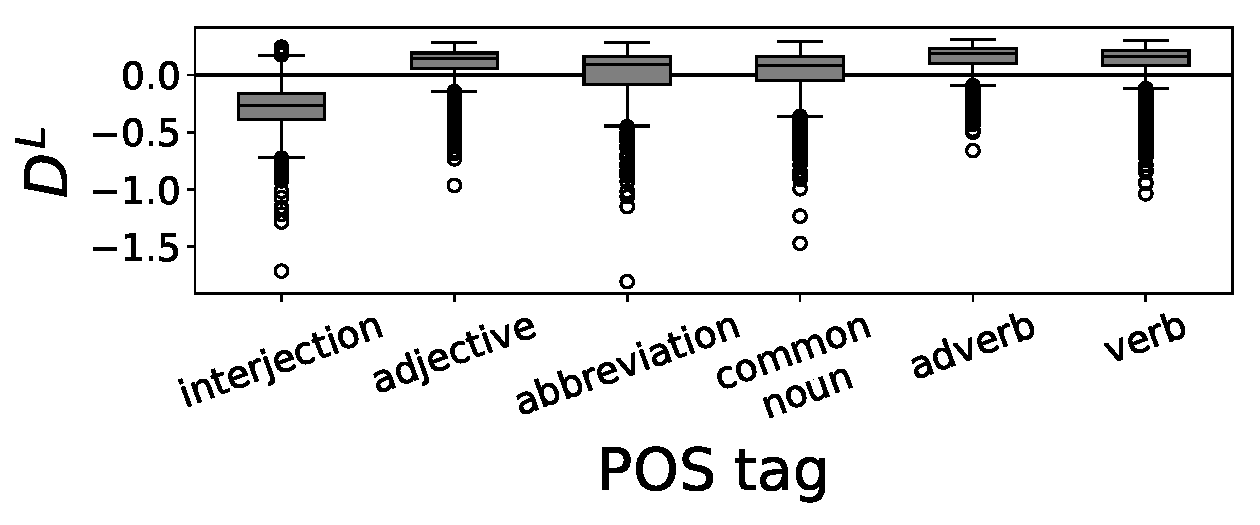
\includegraphics[width=\columnwidth]{figures/pos_DL_distribution.pdf}
\caption{Distribution of mean linguistic dissemination ($D^{L}$) across part of speech groups.}
\label{fig:pos-cd-dist}
\end{figure}

\paragraph{Grammatical aspects of linguistic dissemination}

To confirm the grammatical aspects captured by linguistic dissemination, we visualize the distribution of $D^{L}$ values across words grouped by part of speech tags.
%The grammatical aspects of linguistic linguistic dissemination are confirmed with the distribution of $D^{L}$ across part of speech tags. 
These tags were obtained automatically from the CMU Twitter Part-of-Speech tagger~\cite{gimpel2011}.\footnote{\url{https://github.com/brendano/ark-tweet-nlp} (Accessed 17 June 2017).}
As shown in \autoref{fig:pos-cd-dist}, interjections have lower linguistic dissemination, which follows from being restricted to sentence-initial or sentence-final position. 
In contrast, adjectives and adverbs have high linguistic dissemination because they can appear throughout the sentence, often near open-class words such as nouns and verbs. 
But while these differences are real and in some cases substantial (one-way ANOVA between part-of-speech groups: $F=822.6, p < 0.0001$), robustness checks in ~\autoref{sec:results-binary-predict} show that the role of linguistic dissemination in explaining word growth goes beyond part-of-speech category.

\paragraph{Success prediction: robustness checks}

Considering the uneven distribution of linguistic dissemination across part-of-speech groups (see ~\autoref{fig:pos-cd-dist}), the prediction results may be explained by an imbalance of POS tags between the growth and decline words.
This issue is addressed through two robustness checks: within-group comparison and prediction.

\begin{figure}
\centering
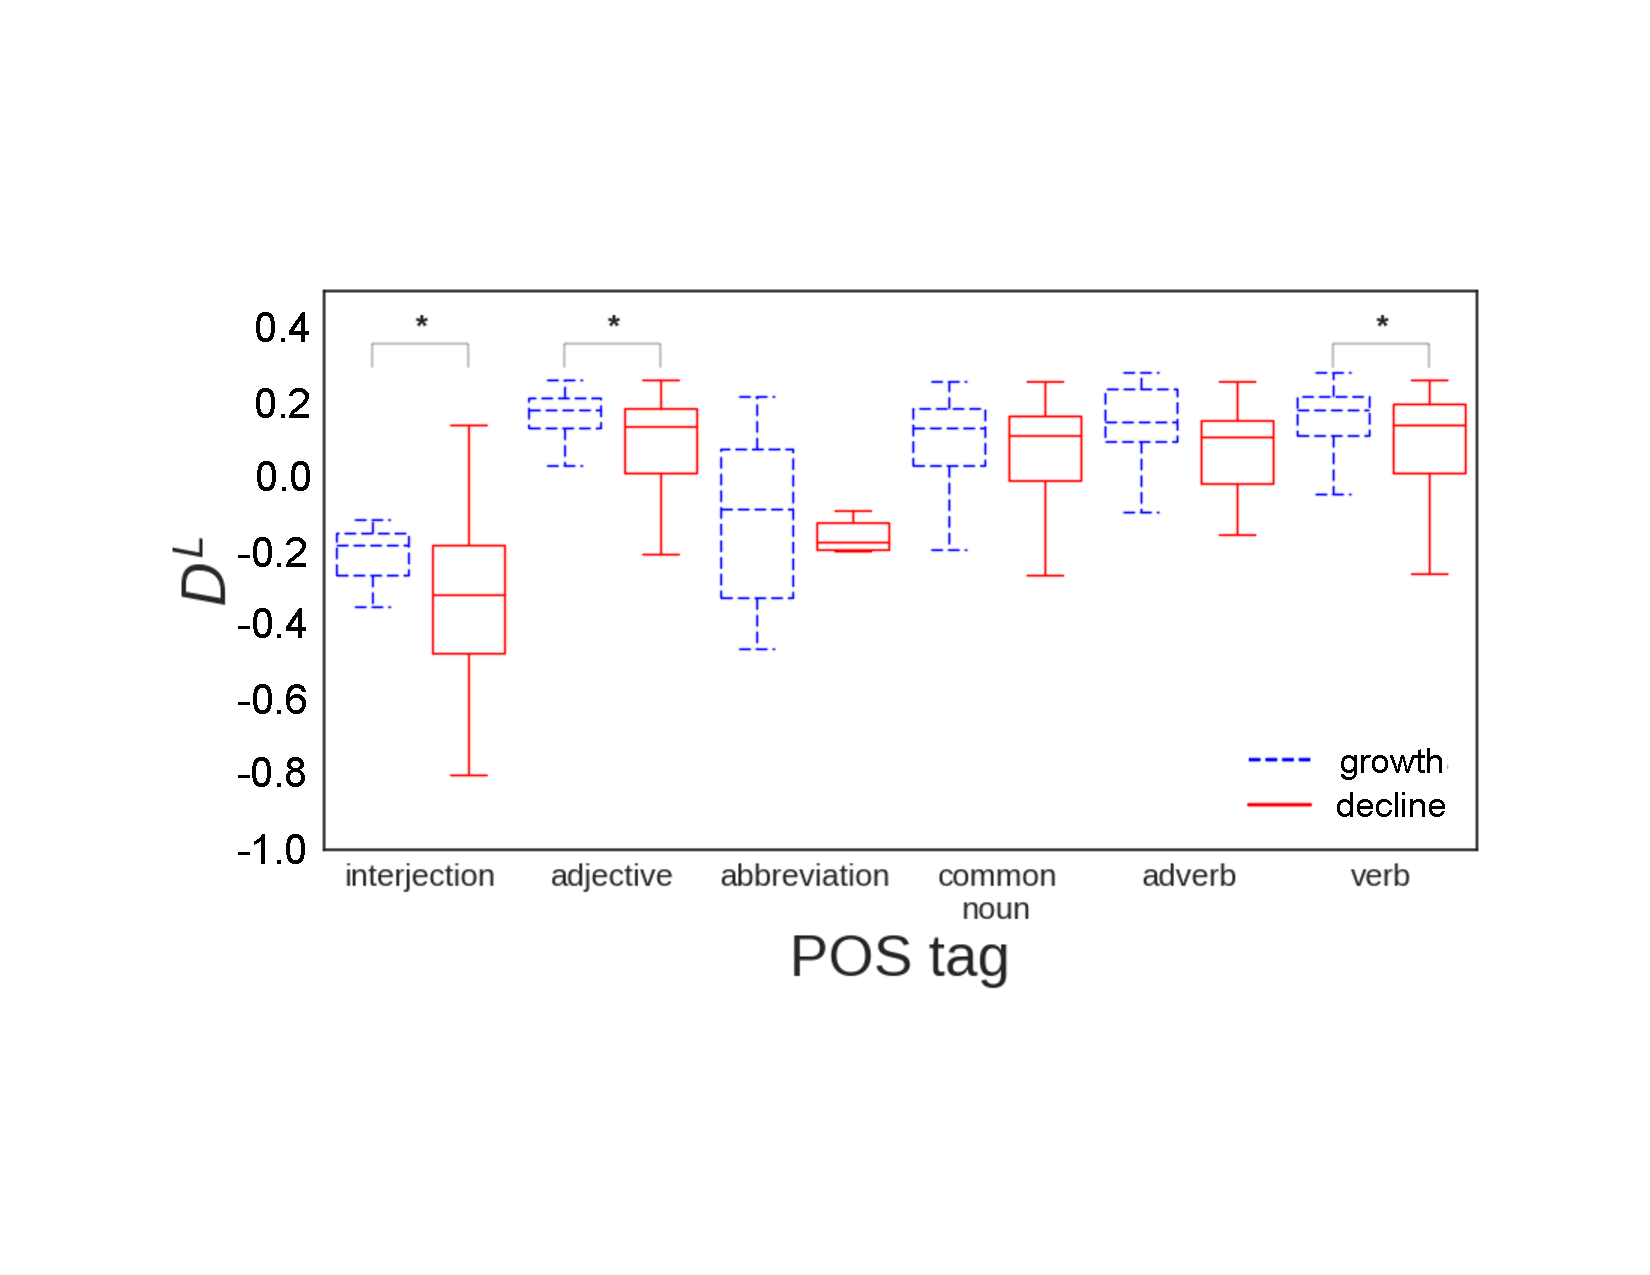
\includegraphics[width=\columnwidth]{figures/growth_vs_decline_matched_pos_DL_distribution_1_12.pdf}
% generated with scripts/frequency/plot_success_vs_failure_pos_DL_distribution.sh
\caption{Distribution of $D^{L}$ values across growth and decline words, grouped by part of speech tag. 
* indicates $p<0.05$ in one-tailed t-test between growth and decline $D^{L}$ values.}
\label{fig:success_vs_failure_pos_DL_distribution}
\end{figure}

First, we compare the distribution of linguistic dissemination values between growth and decline words, grouped by the most common POS tags.
Each decline word is matched with a growth word based on similar mean frequency in the first $k=12$ months, and their mean linguistic dissemination values during that time period are compared, grouped within POS tag groups.
The differences in~\autoref{fig:success_vs_failure_pos_DL_distribution} show that across all POS tags, the growth words show a tendency toward higher linguistic dissemination with significant ($p<0.05$) differences in the interjections and verbs.

Next, the POS tags are used in the same binary prediction task as before, in two different models: (1) as sole features, (2) as additional features in the frequency-only model, each with one month of data ($k=1$).
The linguistic dissemination model significantly outperforms both models (mean accuracy of 50.6\% and 54.8\% respectively), which suggests that the difference in linguistic dissemination between the growth and decline words is not explained by a difference in the POS distribution.

%\begin{figure*}[t!]
%\centering
%\begin{subfigure}[t]{\textwidth}
%\includegraphics[width=\textwidth]{figures/growth_best_fit.pdf}
%\caption{}
%\label{fig:example_time_series_growth}
%\end{subfigure}
%\begin{subfigure}[t]{\textwidth}
%\includegraphics[width=\textwidth]{figures/logistic_decline_best_fit.pdf}
%\caption{}
%\label{fig:example_time_series_decline_logistic}
%\end{subfigure}
%\begin{subfigure}[t]{\textwidth}
%\includegraphics[width=\textwidth]{figures/piecewise_decline_best_fit.pdf}
%\caption{}
%\label{fig:example_time_series_decline_piecewise}
%\end{subfigure}
%\caption{Frequency time series for words from the (a) growth, (b) logistic decline and (c) piecewise decline word sets.}
%\label{fig:example_time_series}
%\end{figure*}
%
%The growth and decline trajectories of the best-fitting words from each word set ($\mathcal{G}, \mathcal{D}_{l}, \mathcal{D}_{p}$; from~\autoref{tab:example_growth_decline_words}) are shown in~\autoref{fig:example_time_series}. 
%The growth words (a) have a clear monotonic growth trajectory, and the decline words (b,c) all follow a similar trajectory of growth up to a peak followed by gradual decline.

\end{appendices}

\end{document}
